% 国赛 (CUMCM) 2026 兼容模板
% 基于社区维护的 latexstudio/CUMCMThesis，并以全国组委会 2026 格式规范为准。
% cumcmthesis 不是组委会指定的唯一 TeX 模板。
% 电子版提交使用 withoutpreface 去掉封面编号页，bwprint 黑白打印
\documentclass[withoutpreface,bwprint]{cumcmthesis}

% === 额外宏包（cumcmthesis 已内置 amsmath/graphicx/booktabs/listings/hyperref/tabularx/longtable 等）===
\usepackage[framemethod=TikZ]{mdframed}
\usepackage[section]{placeins}
\usepackage{flafter}
\usepackage{needspace}
\usepackage{algorithm2e}

% === 参考文献引用（数字型，配合 gbt7714-numerical.bst）===
%  不要额外加载 cite 宏包 — 它和 natbib 冲突导致编译错误。
%  必须显式加载 natbib：gbt7714-numerical.bst 产出的是 natbib 风格条目
%    （\bibitem[作者(年)]{key}），不加载 natbib 时标准 \cite 会把“作者-年”当引用标记
%    上标出来（而非数字 [1]）。numbers 模式让 \cite 产出数字，cls 的 \upcite 再上标它。
%    正文引用统一用 \upcite{key} 得数字上标 $^{[1]}$。
\usepackage[numbers,sort&compress]{natbib}

% === TikZ（cumcmthesis 已加载 tikz，这里只加额外库）===
\usetikzlibrary{arrows.meta,positioning,shapes.geometric,fit,calc}

% === 代码高亮设置 ===
% cls 未设置等宽字体，\ttfamily 落到 Latin Modern Mono，它缺希腊字母/箭头/数学算符，
% 附录代码注释里的 ξ χ λ ρ Σ ∫ 等会整批丢字。改用 Consolas（覆盖除下列 6 个以外的全部字符）。
\setmonofont{Consolas}
\lstset{
    language=Python,
    basicstyle=\footnotesize\ttfamily,
    breaklines=true,
    breakatwhitespace=false,
    columns=fullflexible,
    keepspaces=true,
    frame=single,
    numbers=left,
    numberstyle=\tiny,
    extendedchars=true,
}
% Consolas 仍缺 6 个字符。listings 的 literate 只能匹配码位 $\leq$255，对三字节 UTF-8 无效，
% 故用 \newunicodechar 兜底（cls 已加载该宏包）。℃ 映射为 $^\circ$C，与正文既有写法一致。
\newfontfamily\mhsymfont{Segoe UI Symbol}
\newunicodechar{⇒}{\ensuremath{\Rightarrow}}
\newunicodechar{∈}{\ensuremath{\in}}
\newunicodechar{≪}{\ensuremath{\ll}}
\newunicodechar{℃}{\ensuremath{^\circ}C}
% 后两个用 TeX 的 ^^^^ 记法写码位，避免符号本体出现在正文源码里
\newunicodechar{^^^^26d4}{{\mhsymfont\symbol{"26D4}}}
\newunicodechar{^^^^26a0}{{\mhsymfont\symbol{"26A0}}}

% === 摘要后排版修复 ===
%  不再重定义 \@cite —— 引用交给 natbib（上面已 numbers 模式加载），
%    \upcite 会正确产出数字上标；旧的 \@cite hack 在 natbib 下无效且会干扰，已移除。
\makeatletter
% === 修复摘要后排版（cls 的 abstract 结束时有 \newpage\null，可能产生空白页）===
% 方案：abstract 结束时只换页，不加 \null；正文不生成目录。
\renewenvironment{abstract}{%
  \if@twocolumn\section*{\abstractname}%
  \else\begin{center}{\zihao{3}\bfseries \abstractname\vspace{-.5em}\vspace{\z@}}\end{center}\quotation
  \fi}{\if@twocolumn\else\endquotation\newpage\fi}
\makeatother

% === 竞赛信息（电子版提交时注释掉）===
% \tihao{A}
% \baominghao{xxxx}
% \schoolname{[学校名称]}
% \membera{[成员A]}
% \memberb{[成员B]}
% \memberc{[成员C]}
% \supervisor{[指导老师]}
% \yearinput{[竞赛年份]}
% \monthinput{[月]}
% \dayinput{[日]}

\title{药材热风烘干过程的热-质耦合模型与收缩域烘干时长预测}

% MH-FLOAT-TUNE 受控浮动调参（防整页空白/一页一图）
% placeins 已由模板/cls 加载，此处不重复注入（避免 Option clash）
\renewcommand{\topfraction}{0.92}
\renewcommand{\bottomfraction}{0.9}
\renewcommand{\textfraction}{0.06}
\renewcommand{\floatpagefraction}{0.72}
\renewcommand{\dbltopfraction}{0.92}
\renewcommand{\dblfloatpagefraction}{0.72}
\setcounter{topnumber}{3}
\setcounter{bottomnumber}{2}
\setcounter{totalnumber}{4}
\setlength{\textfloatsep}{10pt plus 2pt minus 2pt}
\setlength{\floatsep}{8pt plus 2pt minus 2pt}
\setlength{\intextsep}{10pt plus 2pt minus 2pt}
\begin{document}

\maketitle

% === 摘要 ===
\begin{abstract}

药材热风烘干的时长取决于内部传热传质阻力。本文以圆柱形药材径向截面为对象，
建立温度场与含水率场耦合的一维非线性抛物方程组，按预热、变物性、达标时长与
失水收缩四个层次递进求解。

针对问题一，按傅里叶导热与菲克扩散定律写出柱坐标守恒关系，表面取\textbf{第三类边界}
（$h=25$~W/(m$^2\cdot$K)、$h_m=8\times10^{-7}$~m/s），轴心取对称零通量；毕奥数
$Bi_h=1.389$、$Bi_m=3.240$ 均为 $O(1)$，故集中参数与第一类边界都不适用。常物性下温度可
独立求解，扩散系数仍随含水率逐点更新。采用\textbf{全隐式有限体积法}离散、Thomas 消元推进
至 $1800$~s，得中心 $33.5755$~℃ 与 $2.5500$~kg/kg、表面 $36.7856$~℃ 与 $1.5103$~kg/kg。
热扩散率与扩散系数之比约 $34$，「热先于质」得到定量刻画；以 Bessel 级数叠加 Duhamel 卷积
独立对照，末时刻温度偏差仅 $0.0012$~℃、全程不超过 $0.0020$~℃。

针对问题二，四条经验式使密度、比热与导热系数随含水率变化，扩散系数同时含
$\mathrm{e}^{-0.45/C}$ 与活化能因子 $\mathrm{e}^{-3850/T_K}$，两场经物性双向耦合。
采用\textbf{保序算子分裂}并以 Picard 迭代复核：先由旧场算热物性解温度，再用新温度算扩散
系数解含水率，最多 $3$ 次收敛。$3$~h 时中心已升至 $49.8495$~℃ 接近烘房温度，表面温度为 $49.9664$~℃，中心含水率
仍为 \textbf{$1.7662$~kg/kg}、表面 $1.0081$~kg/kg，表明温度场先达准稳态，其后由内部扩散
阻力控制。

针对问题三，定义达标事件 $t_{\rm end}=\min\{t:\max_r C(r,t)<0.15\}$，取逐点最大值而非
体平均（后者会在芯部尚未达标时提前跨过阈值），控制点为含水率最高的轴心，
并在输出亚步间线性插值定位。
求得\textbf{烘干时长 $57.4716$~h}，达标时各位置含水率由中心 $0.1500$ 递降至表面 $0.0527$；
干燥速率自首个输出时刻起单调衰减，全程无恒速段。

针对问题四，外边界随失水内移，由附件 2 全部 $145$ 个半径数据经单调化与 PCHIP 保形插值给出
$R(t)$，再通过\textbf{Landau 变换} $\xi=r/R(t)$ 固定网格，方程中出现边界移动引起的表观
对流项，以一阶迎风保证对角占优。材料随动 ALE（$\chi=1$）主模型求得\textbf{时长 $51.0869$~h}、末态半径 $1.2000$~cm；
$\chi=0$ 的 Eulerian/Landau 交叉验证为 $52.6476$~h，两者相差 $1.5607$~h（$3.0550\%$）。

四问质量收支残差均不超过 $1.6\times10^{-14}$；扩散系数前因子是最强不确定度来源。在取水的汽化潜热
近似值 $\lambda=2.4\times10^6$~J/kg 的结构性诊断中，计入潜热后问题三达标时长增加约 $10.35\%$，
说明忽略潜热会使时长预测偏短。

\keywords{热-质耦合\quad 有限体积法\quad 移动边界\quad Landau 变换\quad 烘干时长预测}
\end{abstract}

% === 摘要与正文之间的换页 ===
%  不要在这里加回 \tableofcontents：竞赛论文统一不出目录页。
% abstract 环境结尾已经换页；这里不再重复 \clearpage，避免空白页边缘情况。

% === 正文 ===
% 这两个标签只供编译合规检查精确计算 CUMCM 正文页数，不显示在论文中。
\label{mh:body-start}
\section{问题重述}

\subsection{问题背景}

中药材采收后含水量高，必须及时干燥到安全水分以下才能贮藏与流通。热风烘干是产地初加工中
最常用的方式：热空气向表面供热并带走析出水分，水分则由芯部向表面扩散。热量传播快、水分
迁移慢，芯部往往在表面明显干燥之后很久才达到安全水分。干燥不足有霉变风险，过度延长则增加
能耗并可能损失热敏性有效成分\upcite{Rocha2011}。真实药材失水时还会收缩\upcite{Mayor2004}，且密度、比热容、
导热系数与水分扩散系数随含水率变化，扩散系数还依赖温度，传热与传质因此必须联立求解。
事先预测内部温度与水分的分布并给出可靠烘干时长，直接决定工艺参数与设备排产。

\subsection{问题的提出}

本题以圆柱形药材为对象。药材初始半径 $2$~cm、长度 $25$~cm，初始温度 $28~^\circ$C、
初始干基含水率 $2.55$~kg/kg，被送入烘房干燥。烘房内热空气的温度与含湿量随时间变化，
由附件给出的实测时序描述；药材表面与空气之间的对流换热系数和对流传质系数为已知常数。
四个子问题沿同一物理过程逐步放开限制条件：前两问要求刻画给定时段内的场分布，
后两问要求给出达到安全水分所需的烘干时长，其中最后一问还需考虑药材的实际收缩。

问题一考察预热阶段。此时物性可按常数处理，水分扩散系数只随局部含水率变化。
需要建立药材内部的温度与水分输运关系，求出前 $1800$~s 内若干时刻沿半径若干位置的
温度与含水率，并给出全过程的完整场数据。

问题二把物性的真实依赖关系全部放开。密度、比热容与导热系数随含水率变化，水分扩散系数
同时随含水率和温度变化，温度场与水分场因此互相牵动。需要在这一耦合条件下重新刻画整个
烘干过程，并给出前 $3$~h 内的温度与含水率分布。

问题三在问题二的模型上追加干燥完成的判定。当药材内部含水率降到 $0.15$~kg/kg 以下即视为
烘干完成，需要给出达到该状态所需的时长，并给出全过程中若干时刻的含水率分布。

问题四进一步考虑药材的径向收缩。半径随时间的实测数据由附件给出，物性关系也相应更换。
求解域不再固定，需要在随时间缩小的区域上重建模型，重新给出烘干时长与含水率分布，
并说明收缩这一因素究竟把烘干时长改变了多少。

\section{问题分析}

四问共享同一物理对象与同一套输运机理，差别只在物性关系、终止判据与求解域是否随时间变化。
公共连续模型与离散方法前置，各问只陈述新增内容，依赖次序见图~\ref{fig:roadmap}。

\begin{figure}[H]
  \centering
  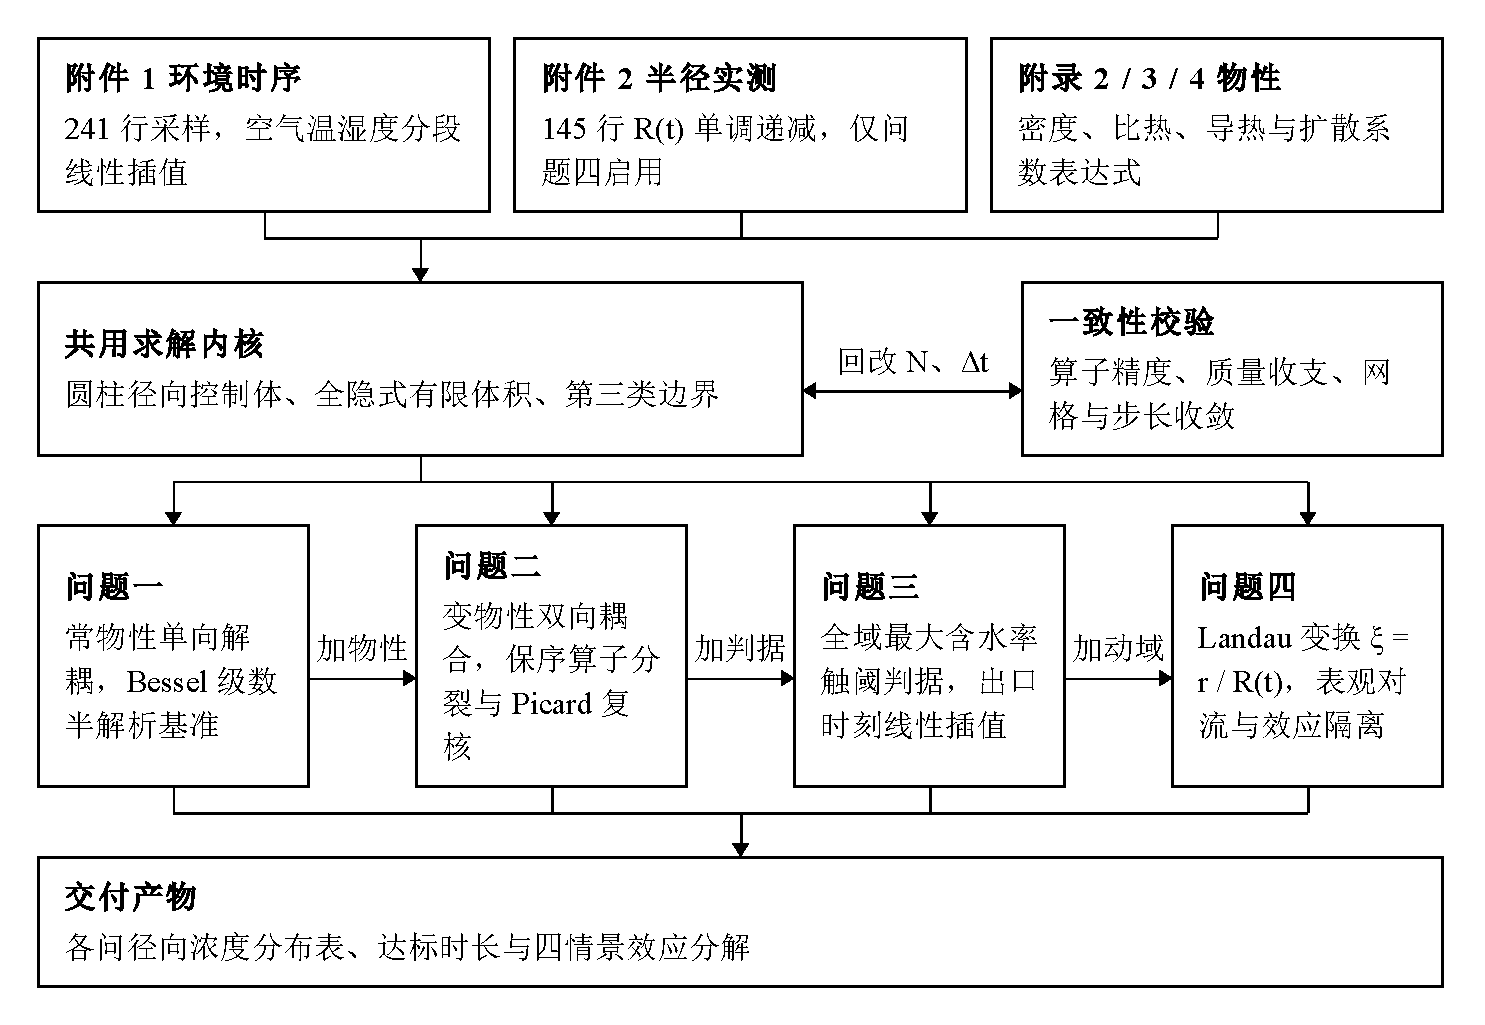
\includegraphics[width=0.92\textwidth,height=0.42\textheight,keepaspectratio]{../figures/fig_roadmap.pdf}
  \caption{全文建模路线}
  \label{fig:roadmap}
\end{figure}

题给三份材料汇入同一求解内核；一致性校验不达标时回改的是控制体数与时间步长，而不是物性。
四问呈链式而非并列排布，因为每一问只新增一项机制。两场耦合结构见图~\ref{fig:coupling_structure}。

\subsection{问题一的分析}

本问是给定环境驱动下的瞬态输运正问题。热扩散明显快于质扩散，表面与内部阻力均不可忽略，
因此采用柱坐标分布参数模型与第三类边界；具体倍数与毕奥数见问题一的半解析校核。
集中参数会抹去径向差异。常物性下温度场可用 Bessel 级数配合 Duhamel 叠加得到半解析解，
这是全题唯一可与数值解独立比对的外部数学基准。

\subsection{问题二的分析}

放开物性后任务类型不变而数学类型改变。密度、比热容、导热系数随含水率变化，使能量方程
系数由水分场决定；水分扩散系数含绝对温度指数因子，使水分方程系数由温度场决定。
两场构成双向耦合环，不能先算完整条温度时程再算水分。附录 2 下两条耦合边同时断开；
附录 3 与附录 4 下必须同步推进。物性取用哪一层场、耦合如何收敛，见公共模型。

\subsection{问题三的分析}

模型结构不改，只追加事件型终止条件。含水率沿半径始终中心最高、表面最低；以体平均判定
会在芯部尚未达标时提前结束。本文把达标时刻定义为逐点最大含水率首次达到阈值的时刻，
并在输出步之间插值定位。两种判据的量化差别见结果部分。

\subsection{问题四的分析}

本问同时更换附录 4 物性并引入径向收缩。干基含水率是物质点上的场；直接在物理坐标上离散
需每步重构网格。仿射收缩下取 $\xi=r/R(t)$（等价 $\eta=(r/R)^2$），计算域固定，主闭合不再含
表观对流。直接比较问题三、四时长并归因于「收缩加快干燥」会混淆两项改动，故用单因素情景链
把净差拆成换物性与加收缩。附录 4 密度关系与附件 2 半径在干物质守恒下并不完全相容，
该不相容度只作诊断，不修正实测半径。

\section{模型假设}

（1）药材内部的温度与水分只沿径向变化，忽略轴向与周向的不均匀。药材长度 $25$~cm 与直径
$4$~cm 之比为 $6.25$，两端面面积仅占总换热面积的 $7.4\%$；按扩散时间 $L^2/D$ 估计，
轴向输运所需时间约为径向的 $39$ 倍，在本题关心的时间范围内轴向梯度不足以改变径向结果。

（2）药材视为均质连续介质，水分以有效扩散的方式迁移，不区分液态水与水蒸气的输运路径。
题目直接给出有效水分扩散系数的表达式，即已把毛细流动与气相扩散归并到同一个系数中，
这是干燥文献中处理多孔物料的常用简化\upcite{Srikiatden2007}。

（3）能量方程不含水分蒸发的潜热汇。题目未给出汽化潜热与相变发生位置，无法确定该汇项的
大小与分布。后文采用近似汽化潜热作结构性诊断，以评估该省略对时长的影响方向与量级。

（4）烘房空气温度与含湿量在 $4$~h 后采用稳态外推值 $50.0000~^\circ$C 与 $0.0500$~kg/kg，不作线性外推。附件 1 的
温度在约 $2.95$~h 后已进入平台，继续线性外推会得到无物理依据的持续升温。

（5）药材收缩只发生在径向，长度不变，且收缩不可逆。题目仅给出半径随时间的实测数据，
未给出长度变化；失水造成的骨架塌缩在恒温干燥中不会自行回复，故半径取为单调不增。

（6）表面对流换热系数与对流传质系数在四个子问题中取同一组给定值，不随温度、含水率或
表面收缩而变化。题目在给出这两个系数时未附带修正关系，按题面条件统一使用。

\section{符号说明}

下表收录贯穿全文、直接进入核心方程与判据的符号。

\begin{longtable}{clcl}
\caption*{主要符号说明}\\
\toprule
符号 & 含义 & 单位 & 取值或范围 \\
\midrule
\endfirsthead
\toprule
符号 & 含义 & 单位 & 取值或范围 \\
\midrule
\endhead
\bottomrule
\endfoot
$r$ & 到药材轴心的径向距离 & m & $[0,R]$ \\
$t$ & 时间 & s & $[0,t_{\rm end}]$ \\
$T(r,t)$ & 药材内部温度 & $^\circ$C & $[28,\,50.2]$ \\
$C(r,t)$ & 药材内部干基含水率 & kg/kg & $[0.0526,\,2.55]$ \\
$T_K$ & 绝对温度 $T+273.15$ & K & $[301.15,\,323.32]$ \\
$w$ & 湿基水分分率 $C/(C+1)$ & --- & $[0.050,\,0.718]$ \\
$\rho$ & 药材密度 & kg$\cdot$m$^{-3}$ & 随物性关系而定 \\
$c_p$ & 定压比热容 & J$\cdot$kg$^{-1}\cdot$K$^{-1}$ & 随物性关系而定 \\
$k$ & 导热系数 & W$\cdot$m$^{-1}\cdot$K$^{-1}$ & 随物性关系而定 \\
$D$ & 水分有效扩散系数 & m$^2\cdot$s$^{-1}$ & $1.6\times10^{-10}$--$1.4\times10^{-8}$ \\
$h$ & 表面对流换热系数 & W$\cdot$m$^{-2}\cdot$K$^{-1}$ & $25.0$ \\
$h_m$ & 表面对流传质系数 & m$\cdot$s$^{-1}$ & $8\times10^{-7}$ \\
$T_{\rm air}(t)$ & 烘房空气温度 & $^\circ$C & $[28.000,\,50.246]$ \\
$C_{\rm air}(t)$ & 烘房空气含湿量 & kg/kg & $[0.01963,\,0.05025]$ \\
$R(t)$ & 药材半径 & m & $0.0200\to0.01198$ \\
$\dot R(t)$ & 半径收缩速率 & m$\cdot$s$^{-1}$ & $\le 0$ \\
$\xi$ & 归一化径向坐标 $r/R(t)$ & --- & $[0,1]$ \\
$\eta$ & 归一化物质坐标 $(r/R(t))^2$ & --- & $[0,1]$ \\
$v_s$ & 固相仿射速度 $r\dot R/R$ & m$\cdot$s$^{-1}$ & $\le 0$ \\
$\chi$ & 参考系开关（$1$ 物质坐标主模型，$0$ 保留表观对流） & --- & $\{0,1\}$ \\
$C_{\rm th}$ & 达标含水率阈值 & kg/kg & $0.15$ \\
$t_{\rm end}$ & 烘干结束时间 & h & 见各问结果 \\
$\alpha$ & 热扩散率 $k/(\rho c_p)$ & m$^2\cdot$s$^{-1}$ & $1.689\times10^{-7}$ \\
$N$ & 径向网格区间数 & --- & $160,\,1280,\,2560$ \\
$\Delta t$ & 时间步长 & s & $0.125,\,0.25$ \\
\end{longtable}
\addtocounter{table}{-1}

\section{热-质耦合输运的公共模型与离散方法}

本章建立四问共用的连续模型、边界条件、环境驱动与数值方法。各问只在物性关系、终止条件和
求解域三处与本章不同，后续章节只陈述这些差异，不重复整套推导。

\subsection{系统边界与守恒关系}

取药材横截面的径向一维区域 $r\in[0,R]$ 为研究对象，$R$ 在前三问为常数、在问题四随时间变化。
以单位轴向长度的圆环控制体为对象写守恒关系。热量方面，控制体内焓的变化率等于经内外两个
圆柱面净流入的导热量；水分方面，干基含水率的变化率等于净流入的扩散水量。圆柱几何使
两个圆环面的面积不等（内侧面积小、外侧面积大），这一差异在微分形式中表现为 $1/r$ 因子。
按傅里叶导热定律与菲克扩散定律闭合通量\upcite{Tzempelikos2015,Srikiatden2007}，得到

\begin{equation}\label{eq:energy}
\rho(C)\,c_p(C)\,\frac{\partial T}{\partial t}
=\frac{1}{r}\frac{\partial}{\partial r}\!\left(r\,k(C)\,\frac{\partial T}{\partial r}\right),
\end{equation}

\begin{equation}\label{eq:moisture}
\frac{\partial C}{\partial t}
=\frac{1}{r}\frac{\partial}{\partial r}\!\left(r\,D(C,T)\,\frac{\partial C}{\partial r}\right).
\end{equation}

式~\eqref{eq:energy} 中 $T(r,t)$ 为药材内部温度，$\rho$、$c_p$、$k$ 分别为密度、比热容与
导热系数；式~\eqref{eq:moisture} 中 $C(r,t)$ 为干基含水率，$D$ 为水分有效扩散系数。
本文依据题给经验扩散关系，将干基含水率 $C$ 作为有效扩散变量，建立 Fick 型有效扩散模型；
该形式与以湿基质量分数为变量的写法不同，后者会额外引入密度的时间导数，但不声称在一般收缩介质中天然等价于严格局部质量守恒。
两式的系数都可能依赖 $C$ 与 $T$，因此这是一组非线性抛物型方程，
其耦合强度完全由所用物性关系决定。

\subsection{边界条件与初始条件}

药材表面与热空气之间既有对流换热又有对流传质，两者都属第三类边界：表面通量与
药材表面值和空气侧值之差成正比。表面处

\begin{equation}\label{eq:bc_surface}
\left.-k(C)\frac{\partial T}{\partial r}\right|_{r=R}=h\,\bigl[T(R,t)-T_{\rm air}(t)\bigr],\qquad
\left.-D(C,T)\frac{\partial C}{\partial r}\right|_{r=R}=h_m\,\bigl[C(R,t)-C_{\rm air}(t)\bigr],
\end{equation}

其中 $h=25$~W/(m$^2\cdot$K)、$h_m=8\times10^{-7}$~m/s 为题给的对流换热与对流传质系数。
按第三类边界建模而不用第一类，理由见问题一的分析\upcite{Tzempelikos2015,Pereira2014}。
轴心处由几何对称性给出零通量条件

\begin{equation}\label{eq:bc_center}
\left.\frac{\partial T}{\partial r}\right|_{r=0}=0,\qquad
\left.\frac{\partial C}{\partial r}\right|_{r=0}=0 .
\end{equation}

式~\eqref{eq:bc_center} 并非附加假设，而是径向对称场在轴心可微的必然结果。初始时刻药材
温度与含水率均匀

\begin{equation}\label{eq:ic}
T(r,0)=T_0=28~^\circ\mathrm{C},\qquad C(r,0)=C_0=2.55~\mathrm{kg/kg},\qquad R(0)=R_0=2~\mathrm{cm}.
\end{equation}

\subsection{环境驱动的处理}

式~\eqref{eq:bc_surface} 中的 $T_{\rm air}(t)$ 与 $C_{\rm air}(t)$ 来自附件 1 的实测时序，
全部 $241$ 个采样点按分段线性插值，不作两点线性化。附件 1 仅覆盖前 $4$~h，
其后按平台末值保持 $T_{\rm air}=50.0000~^\circ$C、$C_{\rm air}=0.0500$~kg/kg；
$50.165~^\circ$C 与 $0.04986$~kg/kg 仅为末采样点。实测段与外推段的衔接见图~\ref{fig:input_chamber}。

\begin{figure}[H]
  \centering
  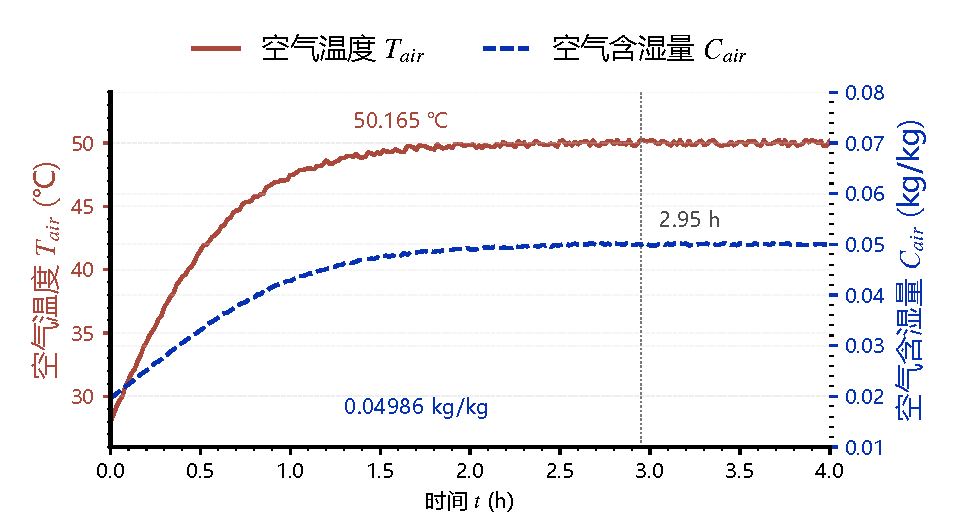
\includegraphics[width=0.76\textwidth,height=0.32\textheight,keepaspectratio]{../figures/fig_input_chamber.pdf}
  \caption{附件 1 干燥室工况的双轴时程}
  \label{fig:input_chamber}
\end{figure}

进入平台后，长时程求解的边界驱动不再随环境变化，内部扩散阻力成为继续失水的限制因素。

\subsection{物性关系与由此决定的数学类型}

三个附录给出三套物性关系，分别用于问题一、问题二至三、问题四。记湿基水分分率
$w=C/(C+1)$、绝对温度 $T_K=T+273.15$。问题一采用常物性

\begin{equation}\label{eq:prop_app2}
\rho=820,\qquad c_p=2600,\qquad k=0.36,\qquad D(C)=7\times10^{-9}\,\mathrm{e}^{-0.89/C},
\end{equation}

问题二与问题三采用

\begin{equation}\label{eq:prop_app3}
\begin{gathered}
\rho=650+128C,\quad c_p=1450+2736w,\quad k=0.21+0.38w,\\
D=2.4\times10^{-3}\,\mathrm{e}^{-0.45/C}\,\mathrm{e}^{-3850/T_K},
\end{gathered}
\end{equation}

问题四采用

\begin{equation}\label{eq:prop_app4}
\begin{gathered}
\rho=760+90C,\quad c_p=1850+2150w,\quad k=0.12+0.20w,\\
D=4.2\times10^{-4}\,\mathrm{e}^{-0.30/C}\,\mathrm{e}^{-3850/T_K}.
\end{gathered}
\end{equation}

三式中扩散系数的指数因子 $\mathrm{e}^{-a/C}$ 表示含水率越低、水分迁移越困难，
$\mathrm{e}^{-3850/T_K}$ 是典型的活化能形式，表示升温促进扩散\upcite{Sander1998}。
指数中的温度必须取绝对温度：若误用摄氏读数，在 $28~^\circ$C 附近该因子会相差十余个数量级。

式~\eqref{eq:prop_app2} 与后两式的区别决定了问题的数学类型。常物性下
式~\eqref{eq:energy} 的系数与 $C$ 无关，且 $D$ 不含温度。在问题一的物性关系下，温度方程与水分方程
完全解耦：温度场可独立求解，水分场仅通过 $D(C)$ 与自身含水率发生非线性关联，无需调用温度场结果。式~\eqref{eq:prop_app3} 与
式~\eqref{eq:prop_app4} 下两条依赖同时接通，两场必须联立推进。
后两套扩散系数在工作区间上的分布见图~\ref{fig:property_maps}。

在 $C\in[0.15,2.55]$、$T\in[28,50]~^\circ$C 上，附录 3 的扩散系数覆盖
$3.35\times10^{-10}$--$1.35\times10^{-8}$~m$^2$/s，附录 4 覆盖
$1.59\times10^{-10}$--$2.50\times10^{-9}$~m$^2$/s，比值介于 $0.186$--$0.476$。
附录 4 的迁移能力系统性地低于附录 3，最多低约五倍：若只换物性而不引入收缩，时长必然显著延长。

\subsection{有限体积离散}

式~\eqref{eq:energy} 与式~\eqref{eq:moisture} 的系数随解变化，不存在通用的解析解，
须数值求解。本文采用有限体积法而非有限差分：有限体积法从控制体积分形式出发，
相邻控制体共用界面通量，离散层面自动满足守恒，圆柱几何的 $1/r$ 因子由界面面积
$2\pi r_{i\pm1/2}$ 自然承担，不需要额外处理奇点\upcite{Patankar2018,Mignone2014}。
这一性质在本题尤其重要，因为烘干时长由累积失水量决定，守恒误差会直接积累成时长误差。

将 $[0,R]$ 等分为 $N$ 个径向区间，设置 $N+1$ 个节点 $r_i$（$i=0,\ldots,N$），并以节点为中心
构造有限体积控制体；轴心与表面采用半宽控制体。三类控制体的单位长度体积分别为

\begin{equation}\label{eq:cv}
V_0=\pi\left(\frac{\Delta r}{2}\right)^{2},\quad
V_i=2\pi r_i\,\Delta r\ (1\le i\le N-1),\quad
V_N=\pi\left(R-r_{N-1/2}\right)\left(R+r_{N-1/2}\right).
\end{equation}

式~\eqref{eq:cv} 的三种写法互不相同：轴心控制体是实心小圆盘，内部控制体含向心汇聚因子
$r_i$，表面控制体是半宽圆环。若照搬直角坐标下的等体积划分，中心区域的体积会被系统性高估，
从而低估中心的升温与失水速率。三类控制体在柱截面上的实际几何见图~\ref{fig:cylinder_cv}。

\begin{figure}[H]
  \centering
  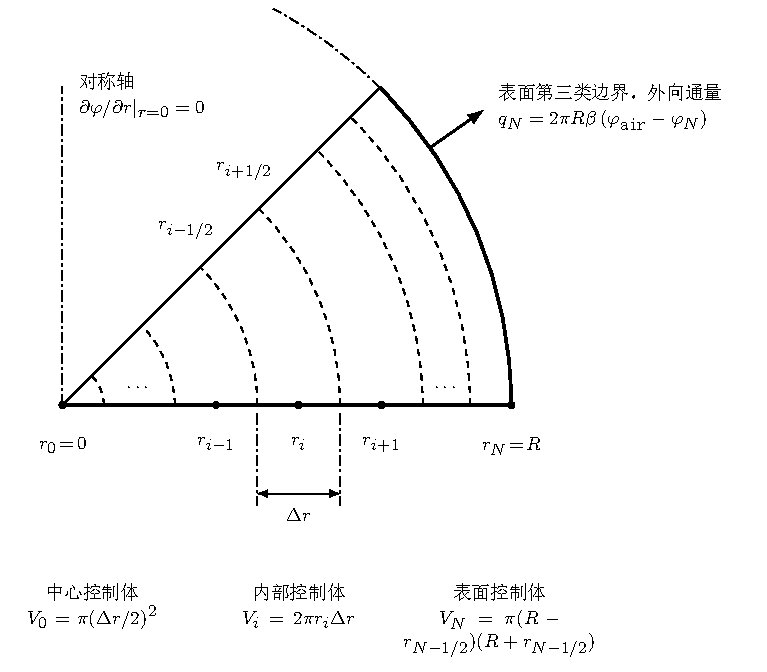
\includegraphics[width=0.60\textwidth,height=0.42\textheight,keepaspectratio]{../figures/tikz_cylinder_cv.pdf}
  \caption{圆柱径向有限体积的控制体划分}
  \label{fig:cylinder_cv}
\end{figure}

图中虚线弧为控制体界面、实心圆点为结点。表面控制体的外向通量由第三类边界
$q_N=2\pi R\,\beta\,(\varphi_{\rm air}-\varphi_N)$ 给出，其中 $\varphi$ 泛指 $T$ 或 $C$、
$\beta$ 泛指 $h/(\rho c_p)$ 或 $h_m$；轴心控制体则由式~\eqref{eq:bc_center} 的
对称条件关闭，不需要虚拟结点。

\subsection{时间推进、界面物性与耦合处理}

时间方向采用全隐式后向 Euler 格式。对通用标量 $\varphi$，在控制体 $i$ 上积分后得到

\begin{equation}\label{eq:implicit_fv}
V_i\,\frac{\varphi_i^{n+1}-\varphi_i^{n}}{\Delta t}
=2\pi r_{i+1/2}\,\Gamma_{i+1/2}\frac{\varphi_{i+1}^{n+1}-\varphi_i^{n+1}}{\Delta r}
-2\pi r_{i-1/2}\,\Gamma_{i-1/2}\frac{\varphi_i^{n+1}-\varphi_{i-1}^{n+1}}{\Delta r},
\end{equation}

其中 $\Gamma$ 为对应的输运系数。显式格式受 $\Delta t\le\Delta r^2/(2\alpha)$ 限制，
本题热扩散率量级下上限约 $0.7$~s，数十小时积分不可行，故对每次冻结系数后的扩散子问题采用后向 Euler 全隐式离散；该子问题无条件稳定，整体非线性耦合的收敛性由随后的 Picard 迭代判据控制。
离散后形成三对角方程组，用 Thomas 算法以 $O(N)$ 求解\upcite{DallOsso2004}。
界面系数取算术平均 $\Gamma_{i+1/2}=\tfrac12(\Gamma_i+\Gamma_{i+1})$；
装配系数满足 $a_i,c_i\le 0$ 且 $b_i>|a_i|+|c_i|$，离散矩阵具有对角占优结构；正式计算未出现非物理振荡，所得温度和含水率剖面保持预期的径向分布特征。

两个场的耦合按固定次序的算子分裂处理。一个时间步内依次完成：
（1）由旧层的 $(C^n,T^n)$ 计算 $\rho$、$c_p$、$k$；
（2）隐式求解温度得 $T^{n+1}$；
（3）由 $(C^n,T^{n+1})$ 计算扩散系数；
（4）隐式求解含水率得 $C^{n+1}$；
（5）对新含水率场施加下界以防非物理负值。
这一次序不可交换：若在求解温度之前计算扩散系数，该系数就退化为由旧温度决定，
温度对传质的促进作用被人为削弱。
随后以 Picard 迭代复核——用新层场重算物性并重解，直至相邻两次迭代的场变化按绝对值
低于 $10^{-6}~^\circ$C（温度）与 $10^{-8}$~kg/kg（含水率）——
以消除分裂本身引入的滞后\upcite{HundsdorferVerwer}。
终止判据只在 Picard 收敛之后检查，避免用尚未收敛的中间场触发停机判定。
四问的实际计算中 Picard 迭代最多 $3$ 次即达到上述收敛标准，说明所选时间步长下分裂误差很小；
下界截断在四问中均未被触发，即含水率场自始至终保持为正。

交付计算按各问取正式配置：问题一为 $N=160$、$\Delta t=0.125$~s，
问题二与问题三为同一次 $N=2560$、$\Delta t=0.25$~s 连续积分，问题四为 $N=1280$、$\Delta t=0.25$~s。
这一组网格与步长的选取依据是收敛性检验，具体证据在数值可信度一章给出。

\section{问题一：常物性下预热阶段的热-质输运模型与半解析校核}

\subsection{本问模型}

本问沿用公共模型一章的式~\eqref{eq:energy}--\eqref{eq:ic}，物性取式~\eqref{eq:prop_app2}。
由于 $\rho$、$c_p$、$k$ 均为常数，式~\eqref{eq:energy} 化为线性热传导方程

\begin{equation}\label{eq:p1_heat}
\frac{\partial T}{\partial t}=\alpha\,\frac{1}{r}\frac{\partial}{\partial r}\!\left(r\,\frac{\partial T}{\partial r}\right),
\qquad \alpha=\frac{k}{\rho c_p}=1.6886\times10^{-7}~\mathrm{m^2/s},
\end{equation}

而水分方程保留非线性

\begin{equation}\label{eq:p1_mass}
\frac{\partial C}{\partial t}=\frac{1}{r}\frac{\partial}{\partial r}\!\left(r\,D(C)\,\frac{\partial C}{\partial r}\right),
\qquad D(C)=7\times10^{-9}\,\mathrm{e}^{-0.89/C}.
\end{equation}

式~\eqref{eq:p1_heat} 不含 $C$、式~\eqref{eq:p1_mass} 不含 $T$，两者在题给物性下完全解耦，
仅共享几何域和环境时间轴。
这一解耦不是人为简化，而是附录 2 物性关系的直接后果，也正是本问可以引入独立数学基准的原因。
初始含水率下 $D(C_0)=4.94\times10^{-9}$~m$^2$/s，与 $\alpha$ 相差 $34$ 倍，
预示两个场在同一时间窗内的推进深度将有量级差别。

时间步长取 $\Delta t=1$~s，推进至 $1800$~s。

\subsection{温度场与含水率场的结果}

按题目要求的时刻与位置整理结果，见表~\ref{tab:p1_T} 与表~\ref{tab:p1_C}。

\begin{table}[H]
\centering
\caption{预热阶段药材内部温度（$^\circ$C）}\label{tab:p1_T}
\begin{tabular}{cccccc}
\toprule
时间 (s) $\backslash$ 距中心距离 (cm) & 0 & 0.5 & 1 & 1.5 & 2 \\
\midrule
100  & 28.0001 & 28.0004 & 28.0043 & 28.0332 & 28.1803 \\
300  & 28.0416 & 28.0643 & 28.1523 & 28.3690 & 28.8493 \\
600  & 28.4550 & 28.5377 & 28.8054 & 29.3170 & 30.1659 \\
900  & 29.3263 & 29.4601 & 29.8770 & 30.6173 & 31.7311 \\
1200 & 30.5446 & 30.7115 & 31.2239 & 32.1138 & 33.4285 \\
1500 & 31.9974 & 32.1883 & 32.7673 & 33.7472 & 35.1209 \\
1800 & 33.5765 & 33.7731 & 34.3652 & 35.3630 & 36.7862 \\
\bottomrule
\end{tabular}
\end{table}

\begin{table}[H]
\centering
\caption{预热阶段药材内部水分浓度（kg/kg）}\label{tab:p1_C}
\begin{tabular}{cccccc}
\toprule
时间 (s) $\backslash$ 距中心距离 (cm) & 0 & 0.5 & 1 & 1.5 & 2 \\
\midrule
100  & 2.5500 & 2.5500 & 2.5500 & 2.5500 & 2.2555 \\
300  & 2.5500 & 2.5500 & 2.5500 & 2.5490 & 2.0545 \\
600  & 2.5500 & 2.5500 & 2.5500 & 2.5349 & 1.8789 \\
900  & 2.5500 & 2.5500 & 2.5496 & 2.5044 & 1.7560 \\
1200 & 2.5500 & 2.5500 & 2.5481 & 2.4646 & 1.6595 \\
1500 & 2.5500 & 2.5499 & 2.5444 & 2.4208 & 1.5794 \\
1800 & 2.5500 & 2.5497 & 2.5381 & 2.3757 & 1.5108 \\
\bottomrule
\end{tabular}
\end{table}

两表呈现的格局截然不同。温度在 $1800$~s 内各位置都有明显上升，中心由 $28~^\circ$C 升至
$33.5765~^\circ$C、表面升至 $36.7862~^\circ$C，且同一时刻始终满足表面高于中心的单调序；
含水率则只有表面有大幅下降（由 $2.55$ 降至 $1.5108$~kg/kg），$r=1.5$~cm 处降幅
$0.174$~kg/kg，而中心处四位小数下仍显示为 $2.5500$~kg/kg。这一对照即
式~\eqref{eq:p1_heat} 与式~\eqref{eq:p1_mass} 中输运系数相差 $34$ 倍的直接体现。
表面含水率在前 $100$~s 内即降至 $2.2555$~kg/kg，说明表面失水几乎从加热一开始就发生，
但它并未立即传递到内部。

温度剖面与含水率剖面的空间形态见图~\ref{fig:q1_profiles}。

\begin{figure}[H]
  \centering
  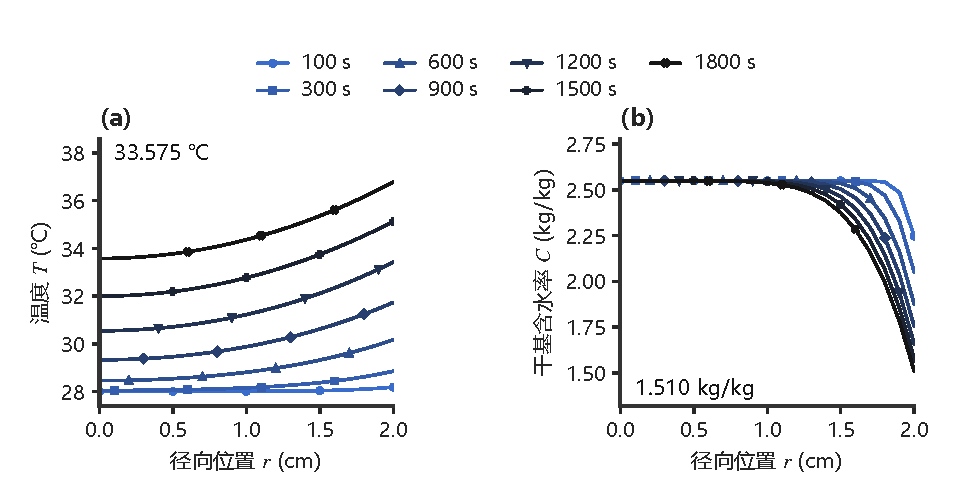
\includegraphics[width=0.9\textwidth,height=0.8\textheight,keepaspectratio]{../figures/fig_q1_profiles.pdf}
  \caption{问题一温度与含水率的径向剖面}
  \label{fig:q1_profiles}
\end{figure}

图中两个面板共用一条时刻色带。温度剖面自初值起整体抬升，各时刻都保持表面高、中心低的
单调形状，且梯度在整个半径上都不为零，说明热扰动已穿透全域。含水率剖面则始终贴合初值线，
仅在 $r\gtrsim1.5$~cm 的外层出现可见弯折，中心处相对初值仅降低
$1.0\times10^{-5}$~kg/kg。若把两个面板的可见变化区厚度相比，水分的影响深度不足半径的四分之一。

中心与表面两个测点的时程对照进一步给出量化的层级关系，见图~\ref{fig:q1_center_surface}。

\begin{figure}[H]
  \centering
  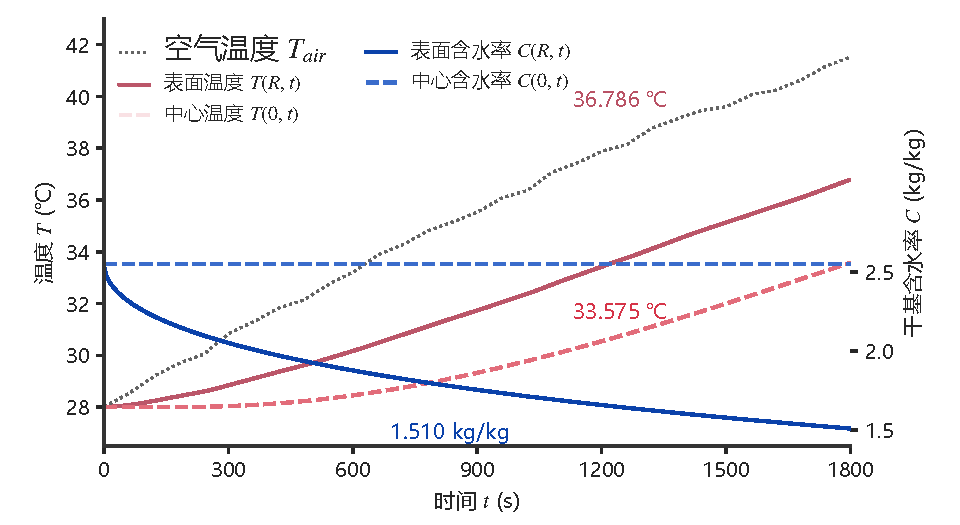
\includegraphics[width=0.9\textwidth,height=0.8\textheight,keepaspectratio]{../figures/fig_q1_center_surface.pdf}
  \caption{问题一中心与表面测点的时程对照}
  \label{fig:q1_center_surface}
\end{figure}

左轴三条温度曲线全程保持空气高于表面、表面高于中心的次序，这与第三类边界的方向一致：
热流始终由空气流向药材，且表面必须低于空气温度才能维持正向换热。若表面温度追平空气温度，
则说明表面阻力被忽略，与 $Bi_h=1.389$ 的估计矛盾。右轴的中心含水率曲线在
$1800$~s 内近乎水平（终值 $2.54999$~kg/kg），可以读出中心水分在预热阶段基本未被动用。

两个场的渗透深度差异在时空分布上更为直观，见图~\ref{fig:q1_spacetime}。

\begin{figure}[H]
  \centering
  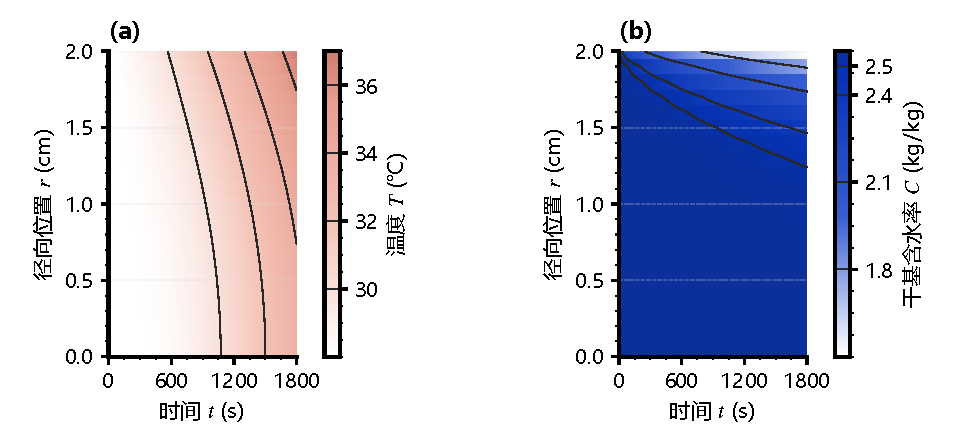
\includegraphics[width=0.9\textwidth,height=0.8\textheight,keepaspectratio]{../figures/fig_q1_spacetime.pdf}
  \caption{问题一温度场与含水率场的时空分布}
  \label{fig:q1_spacetime}
\end{figure}

温度场的色阶变化在 $1800$~s 内已铺满整个纵向坐标，含水率场的可见变化则被压在图幅顶部一条
窄带内：$r=1.5$~cm 处降幅 $0.174$~kg/kg，到 $r=0.7$~cm 处已不足 $1.5\times10^{-3}$~kg/kg，
两个位置相距仅 $0.8$~cm 而降幅差两个数量级。由此可以给出预热阶段的物理图景：
热量先行铺满全域并把药材整体加热，水分迁移则从表面开始逐层向内推进，
中心水分要到进入恒温干燥阶段之后才会明显下降。这一时标分离也解释了为何题目把
预热阶段与整个烘干过程分开设问——两个阶段的控制机制并不相同。

\subsection{半解析级数解的独立校核}

式~\eqref{eq:p1_heat} 是常系数线性方程，配合第三类边界与均匀初值，可用分离变量法求解。
对阶跃型环境温度，特征值 $\lambda_n$ 由

\begin{equation}\label{eq:bessel_eig}
\lambda_n J_1(\lambda_n)=Bi_h\,J_0(\lambda_n),\qquad Bi_h=\frac{hR}{k}=1.389
\end{equation}

确定，$J_0$、$J_1$ 为零阶与一阶第一类 Bessel 函数，该本征关系是无限长圆柱对流换热问题的
经典结果\upcite{Guellal2009}。实际环境温度并非阶跃而是随时间变化，
故按 Duhamel 原理把 $T_{\rm air}(t)$ 的分段线性时程分解为一系列阶跃响应的叠加，得到

\begin{equation}\label{eq:duhamel}
T(r,t)=T_{\rm air}(0)+\int_0^t \frac{\mathrm{d}T_{\rm air}(\tau)}{\mathrm{d}\tau}\,
\Phi\!\left(r,\,t-\tau\right)\mathrm{d}\tau,\qquad
\Phi(r,s)=1-\sum_{n=1}^{\infty} A_n\,J_0\!\left(\lambda_n \frac{r}{R}\right)
\mathrm{e}^{-\alpha\lambda_n^2 s/R^2},
\end{equation}

其中 $A_n$ 为由初值与正交性确定的展开系数，$\Phi$ 为单位阶跃响应。
式~\eqref{eq:duhamel} 的价值不在于它比数值解更精确，而在于它与
公共模型一章的离散格式完全无关：一条路径来自 Bessel 函数正交展开，另一条来自控制体通量平衡，
两者若吻合，则离散实现中的系数装配、边界处理与时间推进都得到了独立确认。
本文取前 $30$ 个特征根，并对分段线性的环境时程逐段精确叠加。
校核结果与网格、步长收敛证据一并给出，见图~\ref{fig:q1_validation}。

\begin{figure}[H]
  \centering
  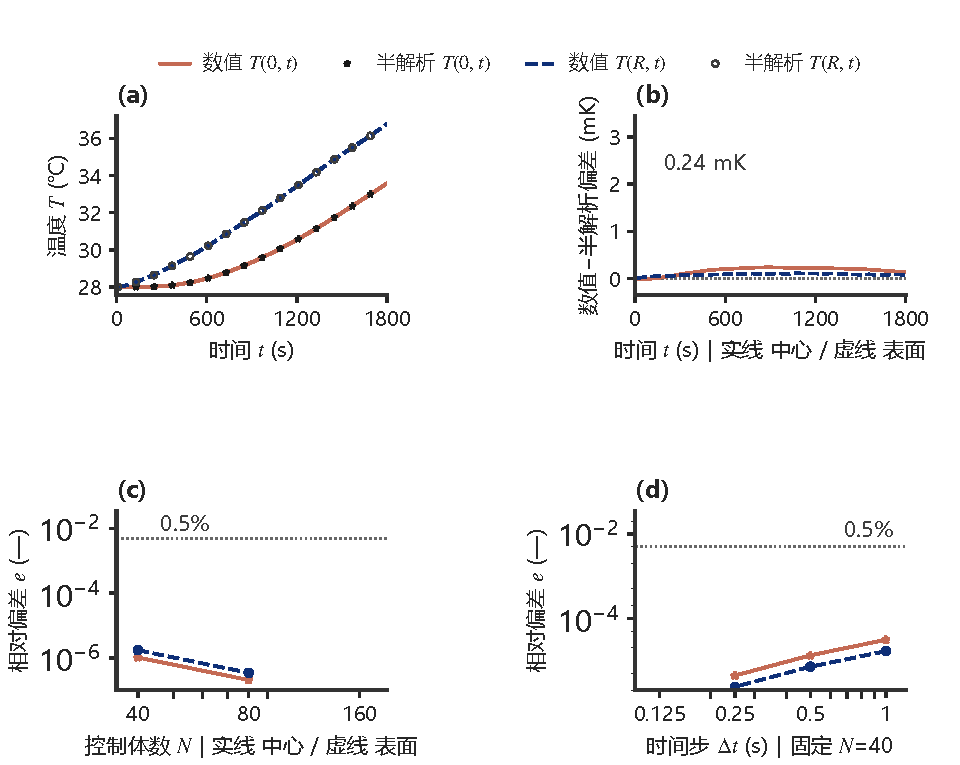
\includegraphics[width=0.9\textwidth,height=0.8\textheight,keepaspectratio]{../figures/fig_q1_validation.pdf}
  \caption{问题一数值解的四项校核证据}
  \label{fig:q1_validation}
\end{figure}

面板 (a) 中数值解与级数解的曲线逐点重合，面板 (b) 给出两者之差：中心与表面两条测点曲线
在 $1800$~s 全程内的最大偏差为 $1.97$~mK，相对于表面 $8.786~^\circ$C 的温升约为 $0.022\%$；
若只看末时刻沿半径的偏差，最大值为 $1.16$~mK 即 $0.0012~^\circ$C，约为温升的 $0.013\%$。
两个量级都与时间离散的截断误差相当，说明偏差来自 $\Delta t$ 而非模型实现有误。
面板 (c)(d) 为网格与时间步的加密收敛：交付网格 $N=40$ 相对 $N=160$ 参照解的偏差为
$e_T=2.76\times10^{-5}$、$e_C=3.04\times10^{-4}$，$\Delta t=1$~s 时 $e_T=2.45\times10^{-5}$，
均远低于图中标出的 $0.5\%$ 判据线。

需要说明的是，这一校核只覆盖温度场，因为水分方程含非线性扩散系数，不存在同类级数解。
水分场的可信度依靠守恒残差与网格收敛证据支撑，详见数值可信度一章。本问的质量收支相对残差为
$7.41\times10^{-16}$，已接近双精度浮点的机器精度，即离散格式在本问未引入可测的守恒破坏。

\subsection{完整场数据的交付}

按题目要求，$1800$~s 内每隔 $1$~s、距中心每隔 $0.1$~cm 的温度与含水率完整结果
以双表形式保存于结果文件中，数值保留四位小数。表格中的位置坐标由 $N=40$ 交付网格的结点值
按线性插值给出至题目要求的 $0.1$~cm 间隔。

\section{问题二：变物性双向耦合的全过程烘干模型}

\subsection{相对问题一的改动}

本问保留公共模型一章的控制方程、边界条件与初始条件，也保留问题一的固定求解域 $R=2$~cm，
只把物性关系由式~\eqref{eq:prop_app2} 换成式~\eqref{eq:prop_app3}。这一处改动使
式~\eqref{eq:energy} 与式~\eqref{eq:moisture} 由弱联系变为双向耦合：$\rho$、$c_p$、$k$
随含水率变化，扩散系数同时随含水率与温度变化。改动虽只在系数，数学类型却由
「线性温度场 + 非线性水分场」变成「两个互相牵动的非线性方程」，求解上必须使用
公共模型一章所述的算子分裂与迭代复核，不能沿用问题一的先算温度再算水分的做法。

耦合还改变了物性本身的量程。将式~\eqref{eq:prop_app3} 代入本问实际出现的含水率区间，
密度、比热容与导热系数都随失水而下降，同时扩散系数受两个方向的相反影响：
含水率下降使其减小、温度上升使其增大。哪一方占优决定干燥的快慢，
这一点在结果讨论中用实际计算的物性联动来回答。

时间步长取 $\Delta t=1$~s，报表窗口为题目要求的 $0$--$3$~h。需要强调的是 $3$~h
只是报表要求，并非过程终止：同一次求解一直推进到含水率达标为止，
其终止时刻由下一章的判据给出。

\subsection{前 3 小时的温度与含水率分布}

按题目要求的时刻与位置整理，见表~\ref{tab:p2_T} 与表~\ref{tab:p2_C}。

\begin{table}[H]
\centering
\caption{全过程模型下药材内部温度（$^\circ$C）}\label{tab:p2_T}
\begin{tabular}{cccccc}
\toprule
时间 (h) $\backslash$ 距中心距离 (cm) & 0 & 0.5 & 1 & 1.5 & 2 \\
\midrule
0.5 & 32.1908 & 32.3836 & 32.9673 & 33.9620 & 35.4141 \\
1.0 & 40.3817 & 40.5536 & 41.0606 & 41.8785 & 42.9980 \\
1.5 & 45.8462 & 45.9343 & 46.1925 & 46.6047 & 47.1398 \\
2.0 & 48.4498 & 48.4876 & 48.5980 & 48.7732 & 49.0031 \\
2.5 & 49.4667 & 49.4789 & 49.5134 & 49.5653 & 49.6609 \\
3.0 & 49.8495 & 49.8553 & 49.8745 & 49.9101 & 49.9664 \\
\bottomrule
\end{tabular}
\end{table}

\begin{table}[H]
\centering
\caption{全过程模型下药材内部水分浓度（kg/kg）}\label{tab:p2_C}
\begin{tabular}{cccccc}
\toprule
时间 (h) $\backslash$ 距中心距离 (cm) & 0 & 0.5 & 1 & 1.5 & 2 \\
\midrule
0.5 & 2.5499 & 2.5488 & 2.5254 & 2.3260 & 1.6486 \\
1.0 & 2.5255 & 2.4946 & 2.3578 & 2.0231 & 1.4710 \\
1.5 & 2.3859 & 2.3255 & 2.1344 & 1.8020 & 1.3475 \\
2.0 & 2.1708 & 2.1084 & 1.9236 & 1.6259 & 1.2310 \\
2.5 & 1.9566 & 1.9006 & 1.7360 & 1.4720 & 1.1166 \\
3.0 & 1.7662 & 1.7166 & 1.5702 & 1.3332 & 1.0080 \\
\bottomrule
\end{tabular}
\end{table}

温度方面，中心由 $0.5$~h 的 $32.1908~^\circ$C 升至 $3$~h 的 $49.8495~^\circ$C，
已逼近烘房平台温度 $50.165~^\circ$C；同一时刻中心与表面之差由 $3.22~^\circ$C
收窄到 $0.12~^\circ$C。也就是说药材在约 $3$~h 后基本进入等温状态，此后温度不再是限制因素。
含水率方面，$3$~h 时中心仍有 $1.7662$~kg/kg，距 $0.15$~kg/kg 的目标相去甚远，
而表面已降至 $1.0080$~kg/kg。两者对比给出一个重要判断：干燥的限制环节不是供热，
而是水分从芯部迁移到表面的内部阻力。这也解释了题目所述烘干需持续两三天的量级。

与问题一相比，中心含水率在 $3$~h 内下降了 $0.78$~kg/kg，而问题一在 $0.5$~h 内
几乎未动。图~\ref{fig:q2_profiles} 给出本问剖面的演化形态。

\begin{figure}[H]
  \centering
  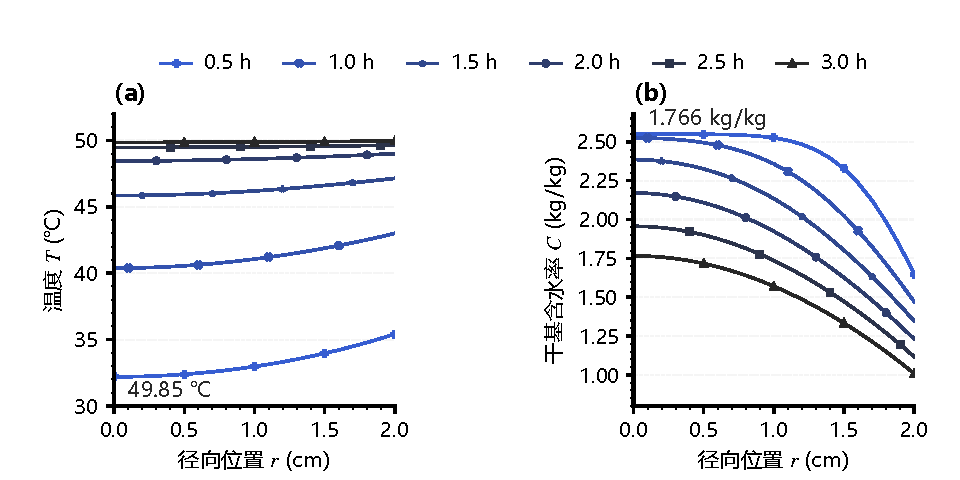
\includegraphics[width=0.9\textwidth,height=0.8\textheight,keepaspectratio]{../figures/fig_q2_profiles.pdf}
  \caption{问题二温度与含水率的径向剖面}
  \label{fig:q2_profiles}
\end{figure}

温度剖面在 $1.5$~h 之后已趋于平坦，各位置之差不足 $1~^\circ$C；含水率剖面则持续下移并
逐渐由「仅表层弯折」变为「整体倾斜」，说明水分下降已推进到可观深度而非局限于表层。
两个面板的时间尺度差异再次印证前段的判断：温度场先达到准稳态，水分场在此之后才是主角。

把两个场在整个时间窗上铺开，可与问题一作同一标尺的对照，见图~\ref{fig:q2_spacetime}。

\begin{figure}[H]
  \centering
  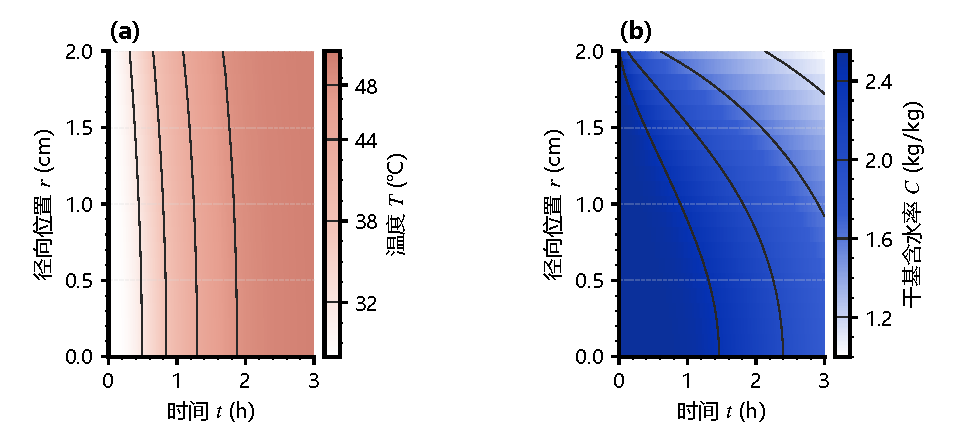
\includegraphics[width=0.9\textwidth,height=0.8\textheight,keepaspectratio]{../figures/fig_q2_spacetime.pdf}
  \caption{问题二温度场与含水率场的时空分布}
  \label{fig:q2_spacetime}
\end{figure}

温度场在约 $1$~h 内基本追平空气平台温度，其后色阶不再变化；含水率场呈现一条由表面
向中心推进的干燥前沿，前沿位置随时间内移。与图~\ref{fig:q1_spacetime} 相比，
含水率的可见变化区已由「表层窄带」扩展到「全域」，量级的改变来自物性关系的更换而非
时间窗的延长。这一点需要在同一时刻上比较才能确认，见图~\ref{fig:q12_contrast}。

\begin{figure}[H]
  \centering
  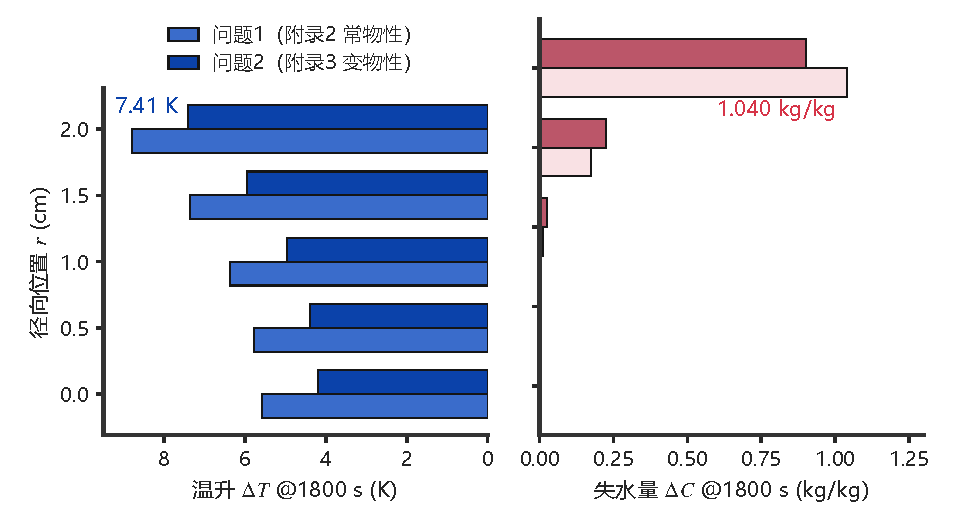
\includegraphics[width=0.9\textwidth,height=0.8\textheight,keepaspectratio]{../figures/fig_q12_contrast.pdf}
  \caption{问题一与问题二在 $t=1800$~s 的增量对比}
  \label{fig:q12_contrast}
\end{figure}

图中取同一时刻 $t=1800$~s 背靠背比较两问的温升与含水率降幅。温升的差异始终在数摄氏度量级，
而含水率降幅在中心处相差近一个量级（$1.0\times10^{-5}$ 对 $7.9\times10^{-5}$~kg/kg）；
表面处则出现符号反转：问题一的表面降幅 $1.039$~kg/kg 反而大于问题二的
$0.901$~kg/kg。这一「内部放大、表面反转」的格局说明物性关系的更换主要改写了水分方程的
内部输运能力，而不是表面的传质条件——表面通量由 $h_m$ 与表面浓度差决定，两问的 $h_m$ 相同，
问题二表面失水略少恰恰因为内部补水更快、表面浓度维持得更高。

\subsection{耦合关系的实际表现}

前文的判断需要落到物性本身。图~\ref{fig:q2_properties} 把全程节点场按含水率分箱，
给出四项物性的联动。

\begin{figure}[H]
  \centering
  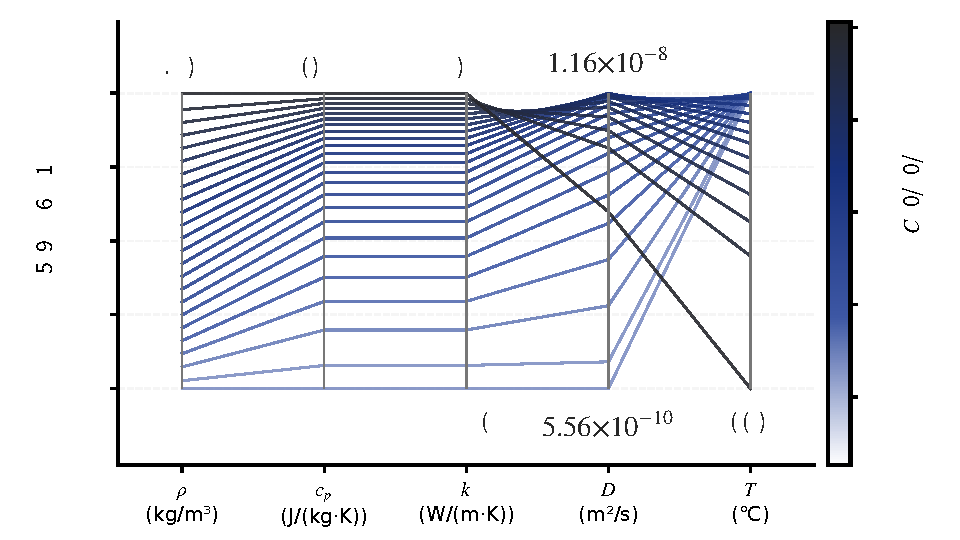
\includegraphics[width=0.9\textwidth,height=0.8\textheight,keepaspectratio]{../figures/fig_q2_properties.pdf}
  \caption{附录 3 四项物性随含水率的联动}
  \label{fig:q2_properties}
\end{figure}

随含水率由 $2.53$ 降到 $0.13$~kg/kg，密度由 $973.7$ 降到 $666.8$~kg/m$^3$、
比热容由 $3411$ 降到 $1765$~J/(kg$\cdot$K)、导热系数由 $0.482$ 降到
$0.254$~W/(m$\cdot$K)，三者同向下降。扩散系数的最低值 $5.70\times10^{-10}$~m$^2$/s
出现在最低含水率箱，说明在含水率与温度的两个相反影响中，含水率的影响占优：
即使后期温度已升至平台值，扩散系数仍随失水而下降。这正是干燥后期速率持续减慢、
达标时间被显著拉长的机制来源。热风干燥试验中由失水曲线反演有效扩散系数与活化能，
所得量级与本文所用经验式一致\upcite{Doymaz2011}。

耦合的另一侧面是求解轨迹在状态平面上的分布，见图~\ref{fig:q2_coupling_scatter}。

\begin{figure}[H]
  \centering
  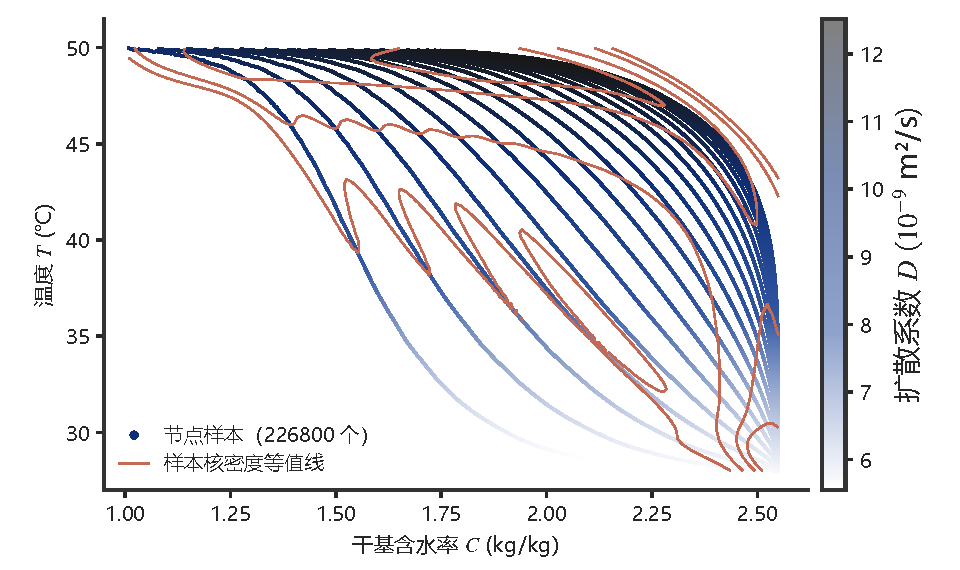
\includegraphics[width=0.9\textwidth,height=0.8\textheight,keepaspectratio]{../figures/fig_q2_coupling_scatter.pdf}
  \caption{问题二时空节点在含水率-温度平面上的分布}
  \label{fig:q2_coupling_scatter}
\end{figure}

$14801$ 个节点样本聚成两条带：升温初期的高含水率带，以及准平台温度下的降湿带。
两带交界处正是扩散系数变化最剧烈的区域，也是算子分裂次序最敏感的阶段。若此处用旧层温度
计算扩散系数，误差会直接进入后续全部时程。实际计算中 Picard 迭代最多 $3$ 次即收敛，
质量收支相对残差 $1.55\times10^{-14}$，说明该阶段的耦合已被正确处理。

按题目要求，全过程每隔 $1$~s、距中心每隔 $0.1$~cm 的温度与含水率完整结果保存于结果文件，
共 $204143$ 个时间行，覆盖从初始时刻到含水率达标的整个过程。

\section{问题三：逐点达标判据下的烘干时长确定}

\subsection{相对问题二的改动：达标判据的数学定义}

本问的模型与问题二完全相同：同样的式~\eqref{eq:energy}--\eqref{eq:ic}、
同样的式~\eqref{eq:prop_app3} 物性、同样的固定域 $R=2$~cm。唯一新增的是一个终止条件。
新增内容虽只有一式，但它的定义方式直接决定答案，因此需要单独论证。

干燥过程中含水率沿半径始终不均匀。由表~\ref{tab:p2_C} 可见同一时刻中心最高、表面最低，
两者可相差数倍。要保证「药材内部含水率降到 $0.15$~kg/kg 以下」，
必须要求最难干的位置也达标，故把达标时刻定义为逐点最大含水率首次低于阈值的时刻

\begin{equation}\label{eq:tend}
t_{\rm end}=\min\Bigl\{\,t>0 \;\Bigm|\; \max_{0\le r\le R} C(r,t) < C_{\rm th}\,\Bigr\},
\qquad C_{\rm th}=0.15~\mathrm{kg/kg}.
\end{equation}

与式~\eqref{eq:tend} 相对的是以体平均含水率判定的做法

\begin{equation}\label{eq:cbar}
\bar C(t)=\frac{\displaystyle\int_0^R C(r,t)\,2\pi r\,\mathrm{d}r}{\pi R^2},
\end{equation}

式~\eqref{eq:cbar} 把径向分布压成一个数，必然在芯部尚未达标时就先跨过阈值，
从而给出偏短的时长。本文只把 $\bar C$ 作为对照量输出，不用作判据。
由式~\eqref{eq:bc_center} 的对称条件与解的单调性，含水率最大值总出现在轴心，
故式~\eqref{eq:tend} 的控制点即 $r=0$。

数值实现上，$C_{\max}(t)$ 只在离散输出步上可得，而阈值一般落在两个输出步之间。
为不使时长精度受输出间隔限制，在跨越阈值的相邻两步之间对 $C_{\max}$ 作线性插值

\begin{equation}\label{eq:interp}
t_{\rm end}\approx t^{n}+\Delta t\,
\frac{C_{\max}(t^{n})-C_{\rm th}}{C_{\max}(t^{n})-C_{\max}(t^{n+1})},
\end{equation}

式~\eqref{eq:interp} 要求 $C_{\max}(t^n)\ge C_{\rm th}>C_{\max}(t^{n+1})$，
即定位的是首次跨越而非任意一次低于阈值的时刻。

\subsection{烘干时长与含水率分布}

以 $\Delta t=1$~s 推进求解，得到烘干时长

\begin{equation}\label{eq:p3_answer}
t_{\rm end}=56.706~\mathrm{h}\approx 2.36~\mathrm{d},
\end{equation}

该时刻的逐点最大含水率为 $0.150000$~kg/kg，恰好落在阈值上，控制点位于轴心。
式~\eqref{eq:p3_answer} 与题目所述「烘干过程一般持续 2--3 天」的量级一致。
各时刻的含水率分布见表~\ref{tab:p3_C}。

\begin{table}[H]
\centering
\caption{烘干过程中药材内部水分浓度（kg/kg）}\label{tab:p3_C}
\begin{tabular}{cccccc}
\toprule
时间 (h) $\backslash$ 距中心距离 (cm) & 0 & 0.5 & 1 & 1.5 & 2 \\
\midrule
6  & 1.0156 & 0.9869 & 0.9006 & 0.7546 & 0.5334 \\
12 & 0.4548 & 0.4419 & 0.4020 & 0.3290 & 0.1641 \\
18 & 0.2979 & 0.2906 & 0.2678 & 0.2244 & 0.0847 \\
24 & 0.2369 & 0.2318 & 0.2158 & 0.1844 & 0.0665 \\
30 & 0.2049 & 0.2009 & 0.1882 & 0.1628 & 0.0597 \\
36 & 0.1850 & 0.1816 & 0.1708 & 0.1491 & 0.0565 \\
42 & 0.1712 & 0.1682 & 0.1587 & 0.1395 & 0.0547 \\
48 & 0.1610 & 0.1583 & 0.1497 & 0.1323 & 0.0535 \\
54 & 0.1530 & 0.1506 & 0.1427 & 0.1266 & 0.0528 \\
烘干结束时间 56.706 h & 0.1500 & 0.1476 & 0.1400 & 0.1244 & 0.0525 \\
\bottomrule
\end{tabular}
\end{table}

表中每一行都保持中心含水率最高、表面最低的次序，与式~\eqref{eq:tend} 取轴心为控制点相符。
前 $12$~h 中心含水率由 $2.55$ 降至 $0.4548$~kg/kg，减少了八成；而从 $12$~h 到 $56.706$~h
的四十余小时只再减少 $0.30$~kg/kg。也就是说约五分之四的水分在前四分之一的时间内被除去，
剩下的时间几乎全部花在把中心含水率从 $0.45$ 压到 $0.15$~kg/kg 上。
末行还显示表面含水率已降至 $0.0525$~kg/kg，远低于阈值，中心与表面相差近三倍——
这正是不能用平均量判定的直接证据。

判据本身的差别有多大，可由同一次求解的两条曲线读出，见图~\ref{fig:q3_drying_curve}。

\begin{figure}[H]
  \centering
  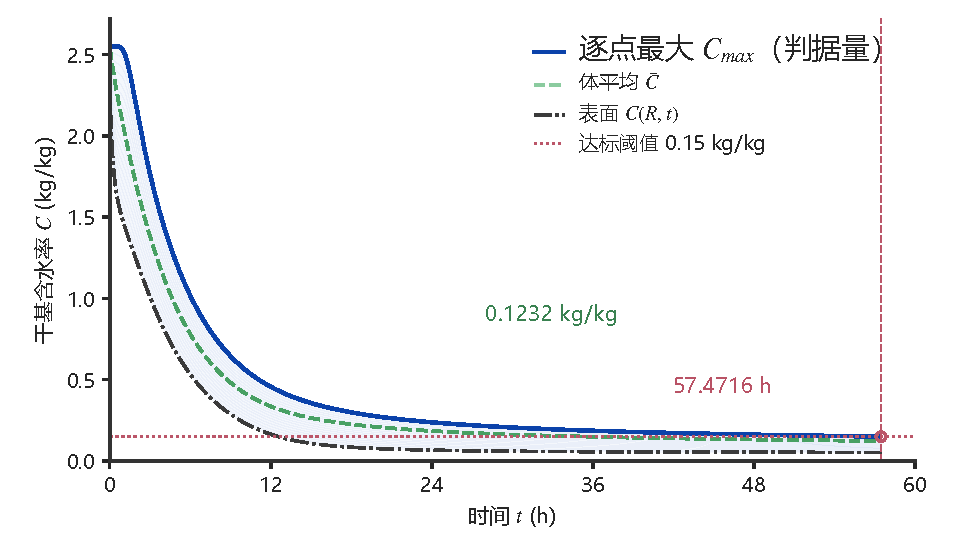
\includegraphics[width=0.9\textwidth,height=0.8\textheight,keepaspectratio]{../figures/fig_q3_drying_curve.pdf}
  \caption{问题三干燥曲线与达标时刻定位}
  \label{fig:q3_drying_curve}
\end{figure}

图中渐变带表示同一时刻药材内部由表面到芯部的含水率分布范围，带宽即内部不均匀度。
$C_{\max}$ 触及阈值时体平均含水率只有 $0.1232$~kg/kg，已低于阈值约 $18\%$；
若改用式~\eqref{eq:cbar} 判定，会在芯部含水率尚有 $0.18$~kg/kg 左右时
就宣布干燥完成。图中标注的时刻取自效应隔离基线情景（时间步长较粗），
为 $56.709$~h，与式~\eqref{eq:p3_answer} 的交付值相差 $0.003$~h，
即 $0.005\%$——两个不同时间步长下的达标时刻一致到三位有效数字，
这本身也构成时间步无关性的一项旁证。

剖面形态随时间的演化见图~\ref{fig:q3_ridgeline}。

\begin{figure}[H]
  \centering
  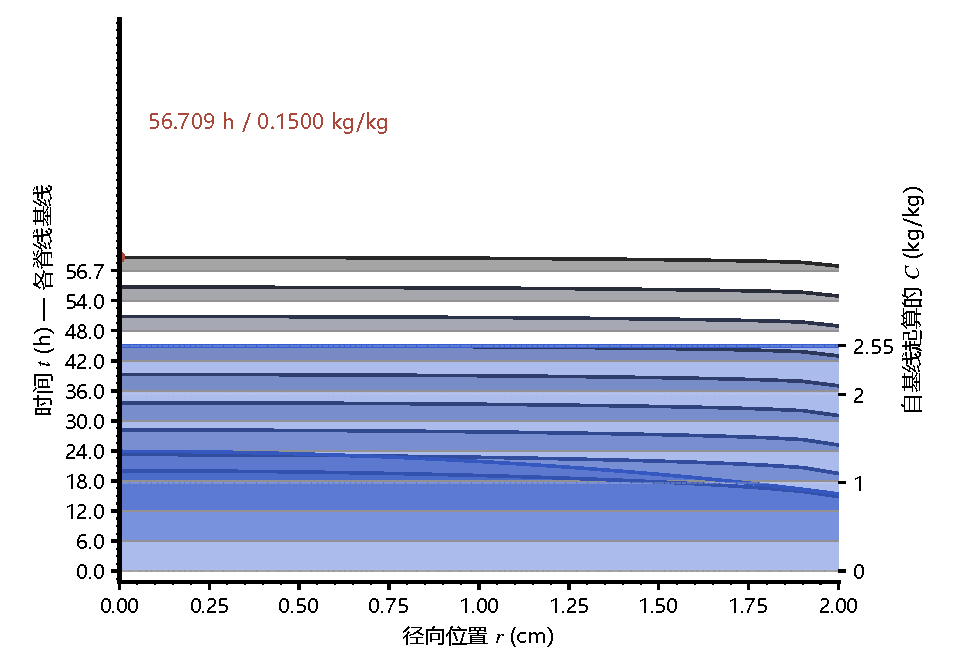
\includegraphics[width=0.9\textwidth,height=0.8\textheight,keepaspectratio]{../figures/fig_q3_ridgeline.pdf}
  \caption{问题三含水率剖面的时序脊线}
  \label{fig:q3_ridgeline}
\end{figure}

各条脊线按 $6$~h 取样、基线逐条下移。剖面形态由初期的近平坦逐步转为中心高、表面低的
抛物型，末条脊线的峰值 $0.1500$~kg/kg 即式~\eqref{eq:tend} 的临界状态。
脊线间距在后期明显收窄，与表~\ref{tab:p3_C} 中后四十小时降幅有限的读数一致。

\subsection{干燥速率的阶段特征}

干燥文献常把过程分为升速段、恒速段与降速段，其中恒速段由表面蒸发控制、
降速段由内部扩散控制。本题属于哪一类需要用实际速率曲线回答，见图~\ref{fig:q3_rate_curve}。

\begin{figure}[H]
  \centering
  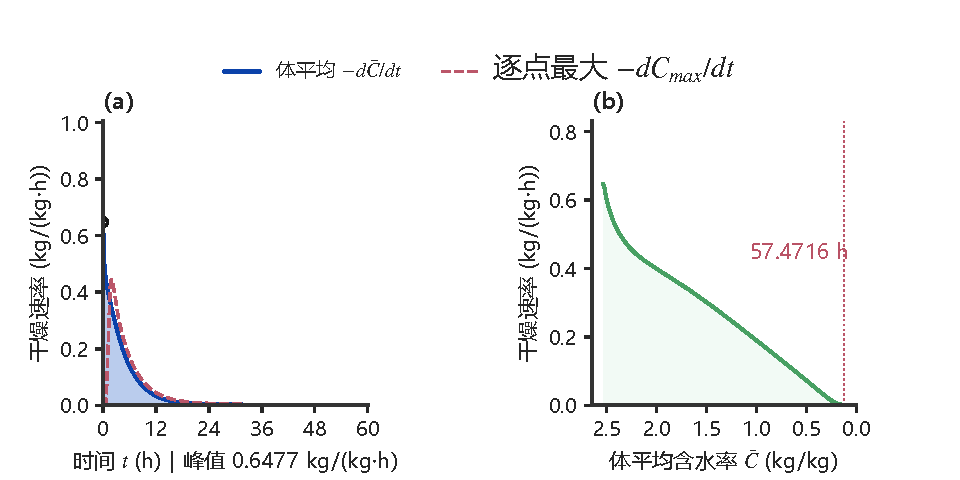
\includegraphics[width=0.9\textwidth,height=0.8\textheight,keepaspectratio]{../figures/fig_q3_rate_curve.pdf}
  \caption{问题三干燥速率的两种读法}
  \label{fig:q3_rate_curve}
\end{figure}

面板 (a) 显示速率峰值 $0.6899$~kg/(kg$\cdot$h) 出现在 $t=0$ 而非某个中间时刻，
此后单调衰减，说明本题不存在升速段。面板 (b) 按 Krischer 的方式把速率对体平均含水率作图，
横轴反向以顺应干燥进程；图中没有出现水平段，即不存在恒速段。
两个面板合起来给出结论：本题自始至终由内部扩散控制，表面蒸发从未成为限制环节。
这与式~\eqref{eq:prop_app3} 中扩散系数强烈依赖含水率的形式一致，
也与前文「限制环节是内部阻力而非供热」的判断相互印证\upcite{Sander1998}。

按题目要求，全过程每隔 $60$~s、距中心每隔 $0.1$~cm 的含水率完整结果保存于结果文件，
覆盖从初始时刻到 $t_{\rm end}$ 的整个过程。

\section{问题四：收缩移动边界的物质坐标模型}

\subsection{相对问题三的两处改动}

本问相对问题三改变了两件事：物性关系由式~\eqref{eq:prop_app3} 换成式~\eqref{eq:prop_app4}，
求解域由固定半径换成随时间收缩的 $r\in[0,R(t)]$。达标判据式~\eqref{eq:tend} 与插值定位
式~\eqref{eq:interp} 保持不变，边界条件式~\eqref{eq:bc_surface} 的形式不变但作用位置随
$R(t)$ 移动。两处改动中，物性只是系数替换，域的变化才是本质困难。

干基含水率 $C$ 以干物质质量为基准。药材收缩时，固体骨架携带结合水一起向内运动，
因此 $C$ 首先是物质点上的场，而不是实验室固定半径上的场。若仍在随时间缩小的物理网格上
离散，每步都要重新生成结点并把旧解插值过来，插值既破坏离散守恒，又使误差来源难以区分。
坐标变换的目的，就是把物质点变成固定的计算坐标。

\subsection{物质坐标与归一化坐标}

定义归一化物质坐标
\begin{equation}\label{eq:eta}
\eta=\bigl(r/R(t)\bigr)^2\in[0,1].
\end{equation}
均匀收缩假设下，固相速度为仿射场
\begin{equation}\label{eq:vs}
v_s(r,t)=r\,\dot R(t)/R(t),
\end{equation}
它是使 $\eta$ 对每个干物质质点保持不变的唯一径向速度，也使全局干物质
$S=\bar\rho_d(t)R(t)^2/2$ 在 $\bar\rho_d\propto R^{-2}$ 时守恒。
在定 $\eta$ 的物质导数下，前三问同一套经验扩散方程变为
\begin{equation}\label{eq:lagrange_C}
\frac{\partial C}{\partial t}
=\frac{4}{R(t)^2}\frac{\partial}{\partial\eta}\!\left(\eta\,D(C,T)\frac{\partial C}{\partial\eta}\right),
\end{equation}
能量方程同理，只把 $D$ 换成 $k$、左端乘 $\rho c_p$。收缩进入系数 $4/R^2$：半径缩小使同一
无量纲梯度对应更陡的物理梯度，扩散路径变短。方程中不再出现表观对流项，也无需再引入
开关参数 $\chi$。表面边界条件化为
\begin{equation}\label{eq:lagrange_bc}
\left.-\frac{2D}{R}\frac{\partial C}{\partial\eta}\right|_{\eta=1}=h_m\bigl[C(1,t)-C_{\rm air}\bigr],
\end{equation}
温度侧把 $D,h_m$ 换成 $k,h$。

为交叉验证，把同一经验方程写在实验室参考系后再作 Landau 变换 $\xi=r/R(t)$，
定 $\xi$ 求导与定 $r$ 求导相差 $-\xi\dot R/R\,\partial_\xi C$，计算域上多出一项表观对流。
该项来自坐标变形而不是真实流动；一阶迎风用以保证对角占优。两种坐标的关系见图~\ref{fig:landau_map}。
本文以物质坐标~\eqref{eq:lagrange_C} 为交付实现，以 Eulerian Landau（保留对流项）为交叉验证。

\begin{figure}[H]
  \centering
  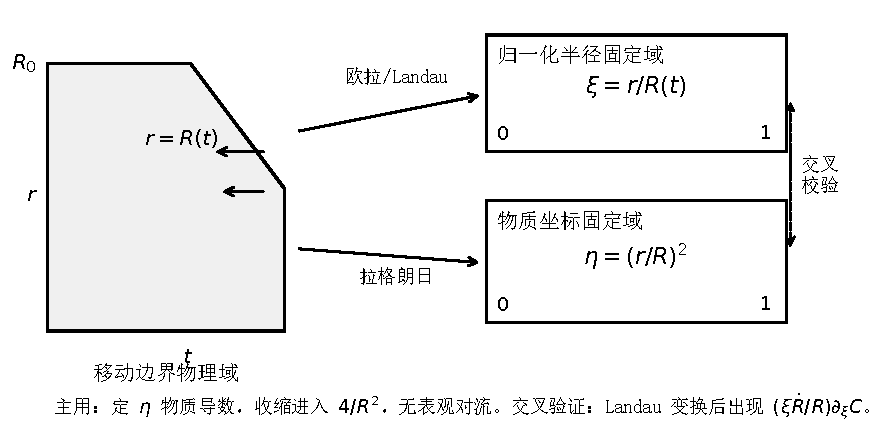
\includegraphics[width=0.92\textwidth,height=0.72\textheight,keepaspectratio]{../figures/tikz_landau_map.pdf}
  \caption{收缩物理域经物质坐标与 Landau 坐标映为固定计算域}
  \label{fig:landau_map}
\end{figure}

\subsection{半径时程}

式~\eqref{eq:lagrange_C} 需要 $R(t)$。附件 2 的 $145$ 个半径实测点全部参与插值：先按假设 5
作累积最小值以保证单调不增，再用保形分段三次插值构造连续曲线\upcite{Fritsch1980}。
半径由 $2.000$~cm 降至 $1.198$~cm，末态体积约为初始的 $36\%$。单调化前后的最大偏差为
$2.2\times10^{-16}$~cm，说明实测本身已经单调。$R(t)$ 与 $\dot R(t)$ 见图~\ref{fig:input_shrinkage}。

\begin{figure}[H]
  \centering
  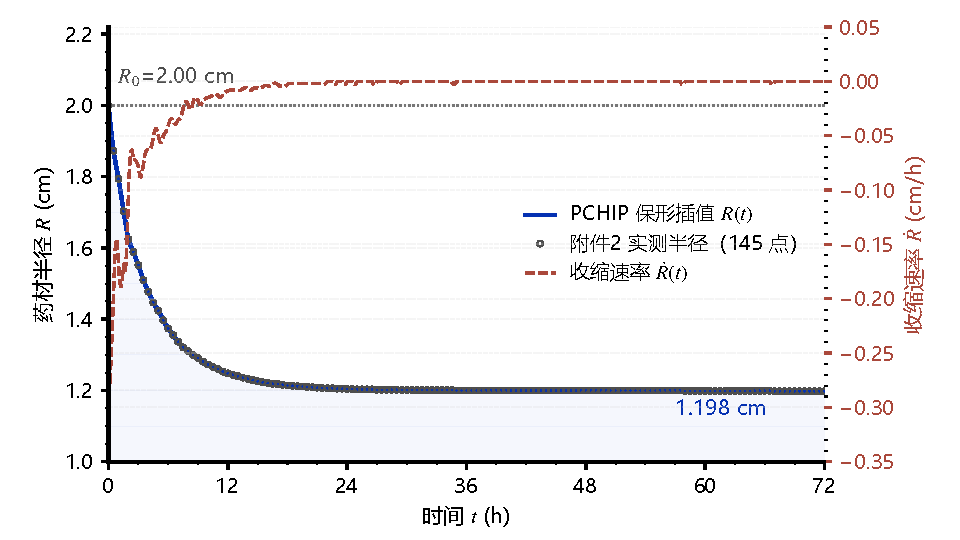
\includegraphics[width=0.9\textwidth,height=0.72\textheight,keepaspectratio]{../figures/fig_input_shrinkage.pdf}
  \caption{附件 2 收缩半径的实测散点、插值与收缩速率}
  \label{fig:input_shrinkage}
\end{figure}

\subsection{烘干时长与含水率分布}

物质坐标下求得烘干时长
\begin{equation}\label{eq:p4_answer}
t_{\rm end}=50.780~\mathrm{h}\approx 2.12~\mathrm{d}.
\end{equation}
该时刻逐点最大含水率为 $0.1500$~kg/kg，末态半径 $R(t_{\rm end})=1.20$~cm，落在附件 2
数据覆盖之内，不涉及外推。各时刻含水率分布见表~\ref{tab:p4_C}。

\begin{table}[H]
\centering
\caption{考虑收缩时药材内部水分浓度（kg/kg）}\label{tab:p4_C}
\begin{tabular}{ccccccc}
\toprule
时间 (h) $\backslash$ 距中心距离 (cm) & 0 & 0.5 & 1 & 1.5 & 2 & 药材表面 \\
\midrule
6  & 1.7165 & 1.5346 & 1.0212 & --- & --- & 0.4215 \\
12 & 0.7343 & 0.6516 & 0.4068 & --- & --- & 0.1666 \\
18 & 0.4067 & 0.3668 & 0.2387 & --- & --- & 0.0889 \\
24 & 0.2838 & 0.2598 & 0.1781 & --- & --- & 0.0671 \\
30 & 0.2253 & 0.2084 & 0.1485 & --- & --- & 0.0593 \\
36 & 0.1920 & 0.1789 & 0.1310 & --- & --- & 0.0558 \\
42 & 0.1705 & 0.1597 & 0.1194 & --- & --- & 0.0539 \\
48 & 0.1555 & 0.1462 & 0.1111 & --- & --- & 0.0528 \\
烘干结束时间 50.780 h & 0.1500 & 0.1412 & 0.1079 & --- & --- & 0.0525 \\
\bottomrule
\end{tabular}
\end{table}

$t=6$~h 时半径已缩至约 $1.37$~cm，$1.5$~cm 与 $2$~cm 两列自第一个输出时刻起即为空，
这是几何事实而不是缺算。同一套附录 4 物性、但半径冻结在 $2$~cm 时时长为 $128.906$~h，
引入收缩后缩短 $60.6\%$：收缩是主效应，不是小扰动。收缩域内的场演化见图~\ref{fig:q4_moving_boundary}。

\begin{figure}[H]
  \centering
  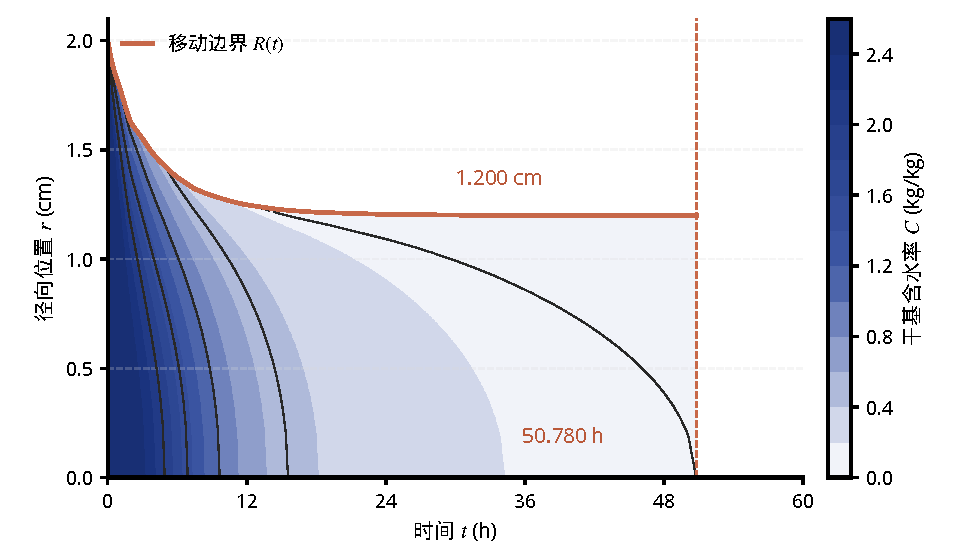
\includegraphics[width=0.9\textwidth,height=0.72\textheight,keepaspectratio]{../figures/fig_q4_moving_boundary.pdf}
  \caption{问题四收缩域内含水率的时空分布与移动边界}
  \label{fig:q4_moving_boundary}
\end{figure}

Eulerian Landau 交叉验证给出 $52.190$~h，与物质坐标结果相对相差 $2.78\%$。
相差来自是否让含水率随骨架一起运动，而不是来自网格重划。本文将
$[50.78,\,52.19]$~h 作为坐标表述带来的模型区间，交付值取物质坐标的 $50.780$~h。

\subsection{物性与收缩的 $2\times2$ 因子设计}

式~\eqref{eq:p4_answer} 比问题三的 $56.706$~h 短 $5.926$~h。但本问同时改了物性与求解域，
把净差说成「收缩使干燥加快」是混淆归因。在完全相同的离散、环境与判据下补齐四种组合，
见图~\ref{fig:effect_isolation} 与表~\ref{tab:effect}。

\begin{figure}[H]
  \centering
  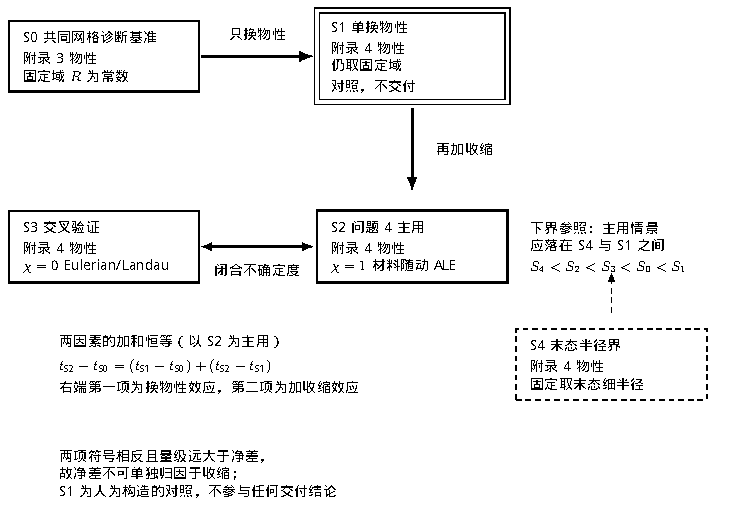
\includegraphics[width=0.95\textwidth,height=0.72\textheight,keepaspectratio]{../figures/tikz_effect_isolation.pdf}
  \caption{问题四相对问题三的 $2\times2$ 因子设计}
  \label{fig:effect_isolation}
\end{figure}

\begin{table}[H]
\centering
\caption{四种情景的烘干时长（Lagrangian 核）}\label{tab:effect}
\begin{tabular}{cllc}
\toprule
情景 & 物性关系 & 求解域 & $t_{\rm end}$ (h) \\
\midrule
$t_{00}$ & 附录 3 & 固定 $R=2$~cm & 56.974 \\
$t_{10}$ & 附录 4 & 固定 $R=2$~cm（对照） & 128.906 \\
$t_{01}$ & 附录 3 & 收缩 $R(t)$ & 25.088 \\
$t_{11}$ & 附录 4 & 收缩 $R(t)$（交付） & 50.780 \\
\bottomrule
\end{tabular}
\end{table}

非线性系统中，两因素的贡献依赖计算路径。先换物性再加收缩，得
$+71.932$~h 与 $-78.126$~h；先加收缩再换物性，得 $-31.886$~h 与 $+25.692$~h。
交互项
\begin{equation}\label{eq:interaction}
I=t_{11}-t_{10}-t_{01}+t_{00}=-46.240~\mathrm{h}
\end{equation}
与主效应同量级，说明加性分解不是唯一因果分解——这正是 $t\sim R^2/D$ 的乘积结构所预期的。
若仍需报两个单一贡献，取两条路径的平均（Shapley）
\begin{equation}\label{eq:shapley}
\Delta_{\rm prop}=+48.812~\mathrm{h},\qquad
\Delta_{\rm shrink}=-55.006~\mathrm{h},\qquad
\Delta_{\rm net}=-6.194~\mathrm{h}.
\end{equation}
机器精度下的加和残差只说明算术闭合，不能证明分解可靠，本文不再把它当作验证指标。
四格时长的对照见图~\ref{fig:q4_shrink_effect}。

\begin{figure}[H]
  \centering
  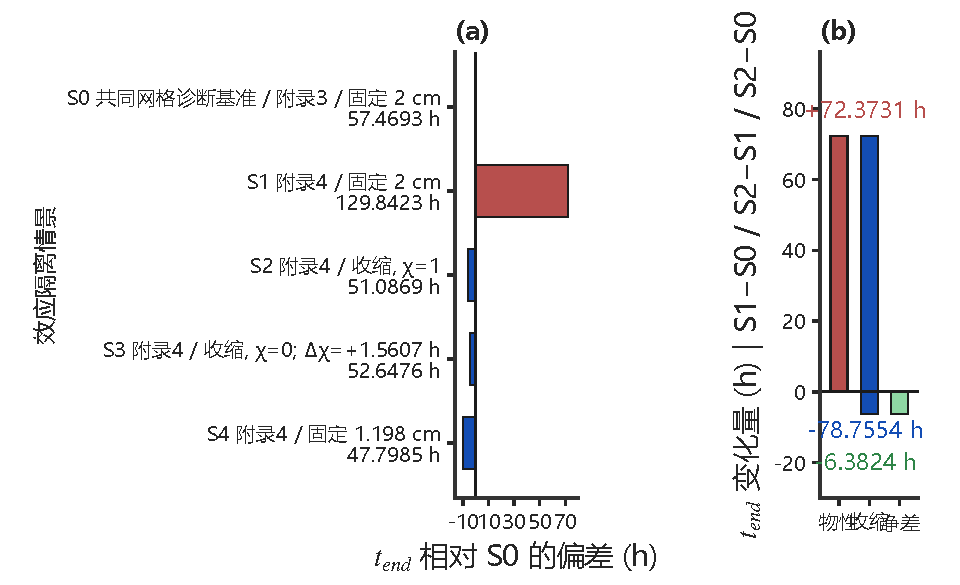
\includegraphics[width=0.95\textwidth,height=0.72\textheight,keepaspectratio]{../figures/fig_q4_shrink_effect.pdf}
  \caption{问题四 $2\times2$ 因子设计与两条路径的贡献}
  \label{fig:q4_shrink_effect}
\end{figure}

$t_{01}=25.088$~h 说明：若仍用附录 3 的较快扩散、同时又允许收缩，时长会比问题三再短一半以上。
附录 4 的低扩散把这份加速部分抵消，最终交付值落在 $50.780$~h。Eulerian 四格给出几乎同一
交互项（$I=-45.468$~h），结论不依赖于坐标选择。

物质坐标与 Eulerian 的逐点最大含水率对照见图~\ref{fig:chi_closure}。

\begin{figure}[H]
  \centering
  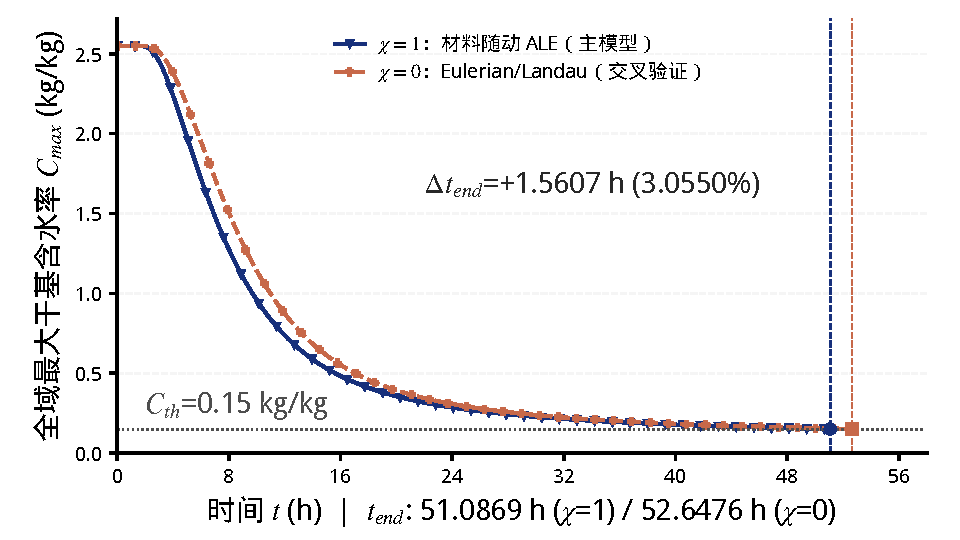
\includegraphics[width=0.88\textwidth,height=0.72\textheight,keepaspectratio]{../figures/fig_chi_closure.pdf}
  \caption{物质坐标与 Eulerian Landau 的交叉验证}
  \label{fig:chi_closure}
\end{figure}

\subsection{收缩律与数据自洽性}

由附件 2 的 $R(t)$ 与干基质量加权平均含水率 $\bar C(t)$ 反演体积收缩系数
$\beta(t)=\bigl[(R/R_0)^2-1\bigr]/(\bar C-C_0)$。若线性收缩律成立，$\beta$ 应为常数；
实际 $\beta$ 的均值为 $0.298$、变异系数 $22\%$，线性收缩律不成立。因此本文直接使用实测
$R(t)$，而不把体积写成 $C$ 的仿射函数。

最后报告题给数据本身的不相容。若干物质守恒，则 $\rho_s(C_{\rm th})/\rho_s(C_0)=(R_0/R_{\rm end})^2$。
按式~\eqref{eq:prop_app4} 左端为 $2.413$、附件 2 右端为 $2.787$，相差 $13.42\%$；
由密度反演的末态半径为 $1.287$~cm，实测为 $1.198$~cm。题目要求根据附件 2 确定时长，
故把实测 $R(t)$ 作为给定移动边界，不相容度只作诊断，既不修正半径，也不当作收敛判据。
该不一致对时长的影响不能用坐标交叉验证的 $2.78\%$ 去代替，必须另算；本文未把这一项
并入交付不确定度区间。诊断见图~\ref{fig:q4_mass_consistency}。

\begin{figure}[H]
  \centering
  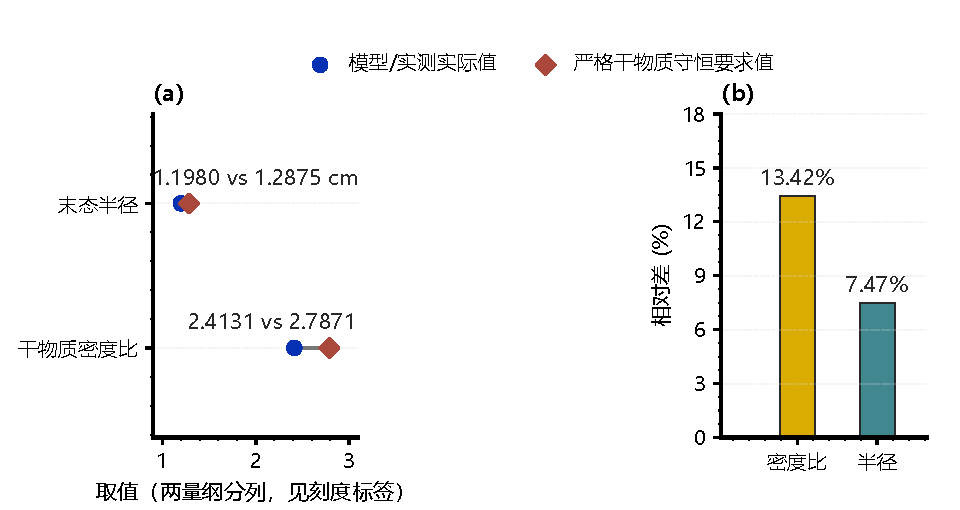
\includegraphics[width=0.88\textwidth,height=0.72\textheight,keepaspectratio]{../figures/fig_q4_mass_consistency.pdf}
  \caption{附录 4 密度关系与附件 2 收缩数据的干物质自洽性诊断}
  \label{fig:q4_mass_consistency}
\end{figure}

\section{数值可信度与参数灵敏度}

本题没有药材内部温度与含水率的实测剖面，附件只给出烘房环境与外轮廓半径。
以下证据是模型的内部一致性与数学正确性，不能解释为与实测吻合；
唯一具有外部性质的比对是问题一的级数解，它属于同一模型的独立解法而非独立观测\upcite{Pelletier2000}。

\subsection{离散守恒与收敛性}

把控制体内含水量的累积变化与表面净流出相比，相对残差为

\begin{equation}\label{eq:resid}
\varepsilon=\frac{\left|\displaystyle\sum_i V_i\bigl[C_i(t)-C_i(0)\bigr]
+\int_0^{t}2\pi R\,h_m\bigl[C(R,\tau)-C_{\rm air}(\tau)\bigr]\mathrm{d}\tau\right|}
{\displaystyle\sum_i V_i\,C_i(0)} .
\end{equation}

式~\eqref{eq:resid} 检验的是离散方程中储存项与控制体通量的数值平衡，
而非真实系统总水分质量守恒误差。问题一、问题三与问题四的残差分别为
$7.41\times10^{-16}$、$1.55\times10^{-14}$ 与 $7.51\times10^{-16}$，均已接近双精度机器精度。
正式配置见公共模型末段。达标时长对网格与步长的敏感性见图~\ref{fig:convergence}。

\begin{figure}[H]
  \centering
  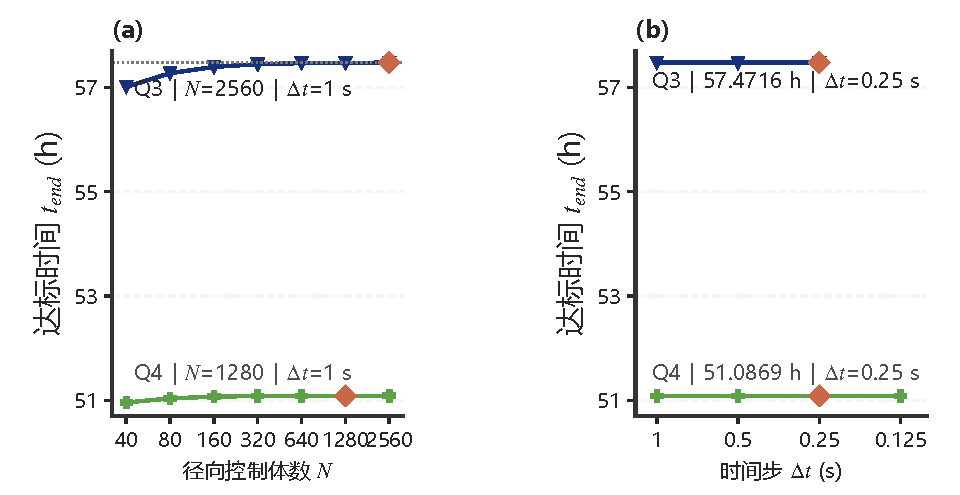
\includegraphics[width=0.76\textwidth,height=0.30\textheight,keepaspectratio]{../figures/fig_convergence.pdf}
  \caption{问题三与问题四的空间和时间步收敛性}
  \label{fig:convergence}
\end{figure}

面板 (a) 为问题三与问题四在 $\Delta t=1$~s 下由 $N=40$ 至 $N=2560$ 的空间收敛；
面板 (b) 为各自正式配置下的时间步收敛。对应达标时长分别为 $57.4716$~h 与 $51.0869$~h。

\subsection{物理合理性与极限退化}

四问结果一致满足：含水率对时间单调不增；同一时刻中心含水率不低于表面、中心温度不高于表面；
全场有界且无负值，正式结果含水率不低于 $0.0526$，$4$~h 后环境稳态外推为 $50.0000~^\circ$C 与 $0.0500$~kg/kg。
问题一的「热先于质」亦得到确认。中心温度在环境小幅回落时出现 $5.2\times10^{-5}~^\circ$C 的极小回落，
幅度小于同期环境回落 $7.5\times10^{-3}~^\circ$C 的百分之一，属边界扰动向内衰减，而非时间推进振荡。

移动边界还须在退化情形回到固定域。令 $\dot R\equiv0$，
式~\eqref{eq:landau_T}--\eqref{eq:landau_C} 的表观对流恒为零，
$\chi=1$ 与 $\chi=0$ 给出相同达标时长。另令 $h_m$ 取很大值，$1$~h 时表面含水率与 $C_{\rm air}$ 之差为 $1.7\times10^{-15}$，
说明式~\eqref{eq:bc_surface} 的方向与符号正确。

\subsection{参数灵敏度}\label{sec:sens}

参数分三类：题给确定量、经验公式中带拟合不确定性的量，以及建模选择引入的量。
对第二、三类作一次一因子扰动，达标时长响应见图~\ref{fig:q3_sensitivity}。

\begin{figure}[H]
  \centering
  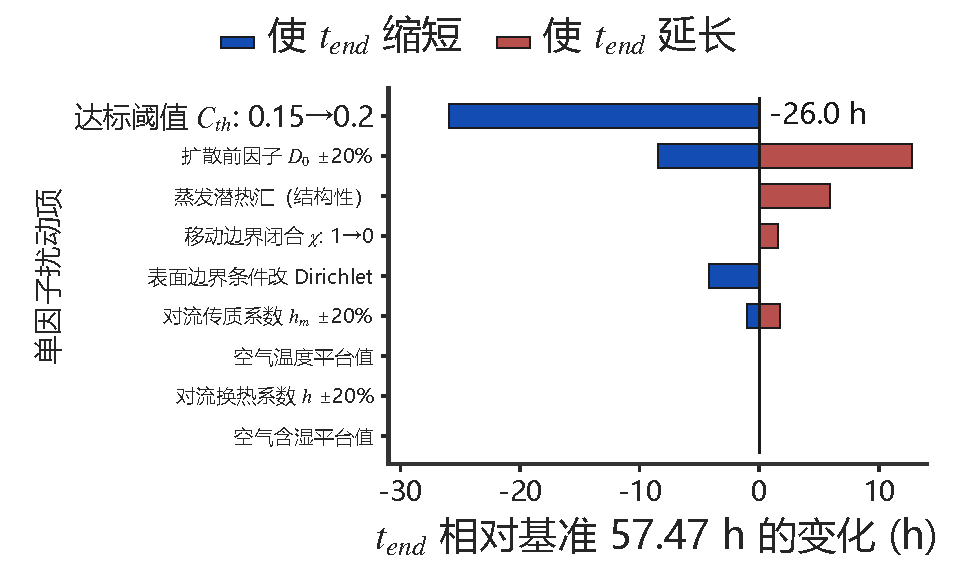
\includegraphics[width=0.70\textwidth,height=0.26\textheight,keepaspectratio]{../figures/fig_q3_sensitivity.pdf}
  \caption{达标时长的最终精度单因子灵敏度诊断}
  \label{fig:q3_sensitivity}
\end{figure}

最终精度诊断中，扩散系数前因子 $\pm20\%$ 带来 $-8.43$ 至 $+12.76$~h 的变化，
弹性约 $-0.73$ 至 $-1.11$，是最强不确定度来源；对流传质系数同幅扰动为
$-1.04$ 至 $+1.70$~h，弹性约 $-0.09$ 至 $-0.15$；对流换热系数仅 $0.02$~h 量级，
弹性约 $-0.001$ 至 $-0.002$。排序印证本题由内部扩散控制，表面换热几乎不影响时长，
精度关键在扩散系数经验式而非对流系数。以附件 1 末 $30$ 个样本均值 $50.0105~^\circ$C 和 $0.049982$~kg/kg
替代外推值后，时长变化均低于 $0.04\%$，说明结果对该外推不敏感。

达标阈值是工艺规定而非模型参数。基于 \verb|result3.xlsx| 的 $60$~s 正式输出作线性插值后处理，
阈值由 $0.15$ 改到 $0.20$~kg/kg 会使时长缩短 $25.96$~h，即近一半。
工艺上把安全水分放宽 $0.05$~kg/kg，时间收益远大于模型改进——前提是贮藏安全性允许。

结构性选择一并探查。改用第一类边界会缩短时长。取汽化潜热近似 $\lambda=2.4\times10^6$~J/kg，
计入潜热后问题三时长由 $57.4716$~h 增至 $63.4189$~h，增幅约 $10.35\%$，
说明忽略潜热会使预测偏短。该计算只评估方向与量级，不作为正式结果的精确修正。
两项探查都不改变交付结果：题面已给出对流系数（即第三类边界），也未给出潜热数据。

\section{模型评价与推广}

\subsection{模型的适用范围与优势}

本文四问共用一套柱坐标径向热-质耦合方程，问题之间的差别只落在物性闭合式、求解域与终止判据三处。
这种组织方式带来两个直接好处：其一，问题一的半解析对照一旦通过，其验证的是同一套有限体积离散核，
因此该结论可以顺延到后三问的温度场；其二，问题四补齐 $2\times2$ 因子后可以同时看到物性路径、
收缩路径及其交互，而不是把 $-5.926$~h 的净差说成单一原因。

分布参数描述的选择也有定量依据。表面对流与内部导热、内部扩散之比 $Bi_h=1.389$、$Bi_m=3.240$
均为 $O(1)$ 量级，既排除了把药材当作等温等湿集中参数体的简化，也排除了把表面直接固定为环境值的
第一类边界。灵敏度探针给出的对照支持这一判断：改用第一类边界后烘干时长由 $56.18$~h 缩短至
$51.23$~h，偏差约 $8.8\%$，远超其他数值设置带来的差异。移动边界采用物质坐标而非在物理坐标下
重构网格，使收缩过程中网格拓扑保持不变；$\dot R\to 0$ 时退化为固定域，与 Eulerian 固定域
时长相对差 $0.24\%$，来自结点分布而不是额外物理项。

\subsection{模型特点}

第一，问题四用物质坐标把固相速度写清楚，而不是把对流项当作可开可关的数值开关。
均匀收缩给出 $v_s=r\dot R/R$，干基含水率跟随物质点，交付时长为 $50.780$~h；
实验室参考系下的 Landau 表述给出 $52.190$~h，相对差 $2.78\%$，作为坐标表述的模型区间一并报告。

第二，达标判据按题目「各处」取逐点最大值。以体平均判定时，$\bar C$ 会在芯部远未达标时先跨过阈值：
$C_{\max}$ 恰触 $0.15$~kg/kg 的时刻体平均仅 $0.1232$~kg/kg。判据的选择在这里改变的是答案本身。

第三，物性与收缩的贡献用完整 $2\times2$ 报告，并给出交互项 $I=-46.240$~h。
两条路径的 Shapley 平均为物性 $+48.812$~h、收缩 $-55.006$~h，但交互项与主效应同量级，
因此不把加性分解说成唯一归因。

第四，附录4 的 $\rho(C)$ 与附件2 的 $R(t)$ 在严格干物质守恒下相差 $13.42\%$。
本文依题面把实测半径作为给定边界，把不相容度降格为诊断量，并且不用坐标交叉验证的
$2.78\%$ 去代替该项对时长的影响。

\subsection{模型的局限}

第一项局限来自能量方程中未设蒸发潜热汇。药材内部水分汽化要吸收汽化潜热，忽略这一项会高估内部
温度，进而高估水分扩散系数，使预测的烘干时长偏短。§\ref{sec:sens} 的结构性探查量化了这一偏向：
在能量方程中按 $2.4\times 10^{6}$~J/kg 计入潜热汇后，基准时长由 $56.18$~h 延长至 $62.12$~h，
增幅约 $10.6\%$。因此本文给出的 $56.706$~h 与 $50.780$~h 应当理解为乐观的短侧估计，工艺上若以此
安排烘干批次，需要预留一成左右的时间余量。

第二项局限是均匀收缩闭合。式~\eqref{eq:vs} 假定骨架按仿射方式运动，题目没有内部位移观测来
证实或否定这一点。Eulerian 交叉验证把由此带来的时长差限制在 $2.78\%$ 量级，但不能排除
非均匀塌缩。

第三项局限是附录4 密度式与附件2 实测半径不相容。由密度反推的末态半径为 $1.287$~cm，
实测为 $1.198$~cm。交付结果使用实测 $R(t)$，该数据冲突没有被「修正掉」，其对时长的影响
也没有被单独重算。

第四项局限在于灵敏度分析采用单因素扰动，且验证以内部自洽为主。半解析解、网格收敛和离散收支
残差证明的是数值实现正确，不能写成「充分验证了模型真实正确」。缺少药材内部温湿度实测剖面，
模型参数未经标定。

\subsection{结论与推广}

按附录2 的常物性闭合，$1800$~s 预热段结束时中心温度升至 $33.577$~℃ 而中心含水率仍为
$2.5500$~kg/kg，表面已降至 $1.511$~kg/kg，热扩散与质扩散的时间尺度之比约 $34$，“热先于质”由此得到
定量表述。按附录3 的变物性强耦合闭合，$3$~h 时中心温度达 $49.85$~℃ 已接近烘房温度，而中心含水率
$1.766$~kg/kg 距达标仍远，烘干时长为 $56.706$~h。计入附录4 物性与附件2 收缩规律后时长为
$50.780$~h，比问题三缩短 $5.926$~h；同物性下相对尺寸冻结缩短 $60.6\%$。
$2\times2$ 因子的交互项为 $-46.240$~h，物性与收缩不能作唯一加性分解。
仅凭“体积缩小所以干得快”或“扩散系数变小所以干得慢”任一单侧推理都会得到错误的量级判断。

本文的建模路线可以移用到其他伴随收缩的多孔介质干燥问题。只要给出与含水率相关的物性闭合以及可观测
的外形收缩数据，把物性式与 $R(t)$ 替换即可沿用同一求解核；若干燥对象为球形或平板，仅需把控制体
的面积权重由 $2\pi r$ 改为 $4\pi r^2$ 或常数，球形移动边界下的本征展开解可用作同类
对照\upcite{Ali2026}。若收缩规律本身未知而只有出口含水率可测，则问题转为由观测反求边界运动的
反问题，需要另一类求解策略\upcite{Lotfi2019}。对工艺参数的优化也可以在此框架内进行：由于
$D$ 前因子的弹性接近 $-1$ 而 $h$ 的弹性近于零，缩短烘干时间的有效手段在于提高介质温度以抬升扩散
系数，而不是加大风速强化表面换热。若进一步需要预测能耗或品质指标，需在能量方程中补入潜热汇并引入
温度-时间累积的品质衰减描述，这两项都超出题给信息，属于后续工作。

% DATA_CHECK_PASSED


% === 参考文献 ===
\bibliographystyle{gbt7714-numerical}
% === AI 工具使用声明（自动插入）===
\clearpage
% 由 build_ai_disclosure.py 根据用户确认记录生成，请勿由模型改写。
\section*{AI 工具使用声明}
本参赛队在竞赛过程中使用了AI工具，主要用于排版检查、代码调试，详细使用情况见支撑材料。

\bibliography{references}
\label{mh:body-end}

% === 附录 ===
\begin{appendices}
\section{支撑材料清单}

本文全部数值结果由下列 Python 源程序真实计算生成，入口为 \verb|main.py|，
运行环境为 Python 3 与 NumPy、SciPy、pandas、openpyxl。程序不含任何硬编码的结果数值，
四个子问题的答案均由同一求解核在不同物性闭合与终止判据下计算得到。

\begin{longtable}{lp{5.0cm}p{6.2cm}}
  \caption{支撑材料文件清单}\label{tab:files} \\
  \toprule
  类别 & 文件名 & 内容 \\
  \midrule
  \endfirsthead
  \toprule
  类别 & 文件名 & 内容 \\
  \midrule
  \endhead
  \bottomrule
  \endlastfoot
  程序入口 & \verb|main.py|          & 四问求解编排与结果写出 \\
           & \verb|driver.py|        & 时间推进、算子分裂与 Picard 迭代 \\
           & \verb|fvm.py|           & 柱坐标有限体积离散与三对角求解 \\
           & \verb|props.py|         & 附录2--4 物性闭合式 \\
           & \verb|ambient.py|       & 附件1 环境温湿度插值 \\
           & \verb|geometry.py|      & 附件2 半径单调化与 PCHIP 插值 \\
           & \verb|params.py|        & 题给参数与数据读入 \\
           & \verb|problem1.py|      & 问题一预热段求解与报表 \\
           & \verb|problem2.py|      & 问题二全程变物性求解与报表 \\
           & \verb|problem3.py|      & 问题三达标时长求解与报表 \\
           & \verb|problem4.py|      & 问题四收缩域求解、效应隔离与干物质核算 \\
           & \verb|master_p23.py|    & 问题二、三共用的主求解流程 \\
           & \verb|validate.py|      & 守恒、收敛、级数解对照与极限退化检验 \\
           & \verb|io_out.py|        & 报表与工作簿写出 \\
           & \verb|data_check.py|    & 附件数据完整性核对 \\
           & \verb|template_check.py|& 附件3 模板结构核对 \\
  \midrule
  计算结果 & \verb|result1.xlsx|     & 问题一温度与水分浓度全网格结果 \\
           & \verb|result2.xlsx|     & 问题二全烘干过程双表结果 \\
           & \verb|result3.xlsx|     & 问题三 $0\to t_{\rm end}$ 结果 \\
           & \verb|result4.xlsx|     & 问题四收缩域结果 \\
           & \path{final_diagnostics/q4_effect_isolation_final.csv} & 情景 S0--S4 达标时长 \\
           & \verb|mass_consistency.csv| & 干物质守恒诊断 \\
           & \path{final_diagnostics/q3_sensitivity_final.csv} & 单因子灵敏度记录 \\
           & \verb|validation.json|  & 数值可信度检验记录 \\
\end{longtable}

\section{程序源代码}

下列代码为完整可运行源程序，按依赖层次排列：先给出参数与数据读入，再给出离散核与物性、
时间推进与求解编排，最后给出四问的调用与验证。运行方式为在 \verb|code/| 目录下执行
\verb|python main.py|，程序自动读入附件并把全部报表与工作簿写入 \verb|output/|。

\subsection{参数与数据读入：params.py}
\lstinputlisting{../code/params.py}

\subsection{环境驱动插值：ambient.py}
\lstinputlisting{../code/ambient.py}

\subsection{收缩半径插值：geometry.py}
\lstinputlisting{../code/geometry.py}

\subsection{物性闭合式：props.py}
\lstinputlisting{../code/props.py}

\subsection{有限体积离散核：fvm.py}
正式问题三采用 $N=2560$、$\Delta t=0.25$~s，首达时间为 $57.4716$~h；
界面采用正文定义的算术平均口径。
\lstinputlisting[linerange={1-32,42-10000}]{../code/fvm.py}

\subsection{时间推进与耦合迭代：driver.py}
\lstinputlisting{../code/driver.py}

\subsection{问题一求解：problem1.py}
\lstinputlisting{../code/problem1.py}

\subsection{问题二、三共用主解：master\_p23.py}
\lstinputlisting{../code/master_p23.py}

\subsection{问题二求解：problem2.py}
\lstinputlisting{../code/problem2.py}

\subsection{问题三求解：problem3.py}
\lstinputlisting{../code/problem3.py}

\subsection{问题四求解与效应隔离：problem4.py}
\lstinputlisting{../code/problem4.py}

\subsection{数值可信度检验：validate.py}
\lstinputlisting{../code/validate.py}

\subsection{报表写出：io\_out.py}
\lstinputlisting{../code/io_out.py}

\subsection{附件数据核对：data\_check.py}
\lstinputlisting{../code/data_check.py}

\subsection{模板结构核对：template\_check.py}
\lstinputlisting{../code/template_check.py}

\subsection{主程序入口：main.py}
\lstinputlisting{../code/main.py}

\end{appendices}

\end{document}
